\documentclass[twoside]{book}

% Packages required by doxygen
\usepackage{fixltx2e}
\usepackage{calc}
\usepackage{doxygen}
\usepackage[export]{adjustbox} % also loads graphicx
\usepackage{graphicx}
\usepackage[utf8]{inputenc}
\usepackage{makeidx}
\usepackage{multicol}
\usepackage{multirow}
\PassOptionsToPackage{warn}{textcomp}
\usepackage{textcomp}
\usepackage[nointegrals]{wasysym}
\usepackage[table]{xcolor}

% Font selection
\usepackage[T1]{fontenc}
\usepackage[scaled=.90]{helvet}
\usepackage{courier}
\usepackage{amssymb}
\usepackage{sectsty}
\renewcommand{\familydefault}{\sfdefault}
\allsectionsfont{%
  \fontseries{bc}\selectfont%
  \color{darkgray}%
}
\renewcommand{\DoxyLabelFont}{%
  \fontseries{bc}\selectfont%
  \color{darkgray}%
}
\newcommand{\+}{\discretionary{\mbox{\scriptsize$\hookleftarrow$}}{}{}}

% Page & text layout
\usepackage{geometry}
\geometry{%
  a4paper,%
  top=2.5cm,%
  bottom=2.5cm,%
  left=2.5cm,%
  right=2.5cm%
}
\tolerance=750
\hfuzz=15pt
\hbadness=750
\setlength{\emergencystretch}{15pt}
\setlength{\parindent}{0cm}
\setlength{\parskip}{0.2cm}
\makeatletter
\renewcommand{\paragraph}{%
  \@startsection{paragraph}{4}{0ex}{-1.0ex}{1.0ex}{%
    \normalfont\normalsize\bfseries\SS@parafont%
  }%
}
\renewcommand{\subparagraph}{%
  \@startsection{subparagraph}{5}{0ex}{-1.0ex}{1.0ex}{%
    \normalfont\normalsize\bfseries\SS@subparafont%
  }%
}
\makeatother

% Headers & footers
\usepackage{fancyhdr}
\pagestyle{fancyplain}
\fancyhead[LE]{\fancyplain{}{\bfseries\thepage}}
\fancyhead[CE]{\fancyplain{}{}}
\fancyhead[RE]{\fancyplain{}{\bfseries\leftmark}}
\fancyhead[LO]{\fancyplain{}{\bfseries\rightmark}}
\fancyhead[CO]{\fancyplain{}{}}
\fancyhead[RO]{\fancyplain{}{\bfseries\thepage}}
\fancyfoot[LE]{\fancyplain{}{}}
\fancyfoot[CE]{\fancyplain{}{}}
\fancyfoot[RE]{\fancyplain{}{\bfseries\scriptsize Generated on Wed Apr 29 2015 11\+:14\+:03 for Voxel Game 2.\+0 by Doxygen }}
\fancyfoot[LO]{\fancyplain{}{\bfseries\scriptsize Generated on Wed Apr 29 2015 11\+:14\+:03 for Voxel Game 2.\+0 by Doxygen }}
\fancyfoot[CO]{\fancyplain{}{}}
\fancyfoot[RO]{\fancyplain{}{}}
\renewcommand{\footrulewidth}{0.4pt}
\renewcommand{\chaptermark}[1]{%
  \markboth{#1}{}%
}
\renewcommand{\sectionmark}[1]{%
  \markright{\thesection\ #1}%
}

% Indices & bibliography
\usepackage{natbib}
\usepackage[titles]{tocloft}
\setcounter{tocdepth}{3}
\setcounter{secnumdepth}{5}
\makeindex

% Hyperlinks (required, but should be loaded last)
\usepackage{ifpdf}
\ifpdf
  \usepackage[pdftex,pagebackref=true]{hyperref}
\else
  \usepackage[ps2pdf,pagebackref=true]{hyperref}
\fi
\hypersetup{%
  colorlinks=true,%
  linkcolor=blue,%
  citecolor=blue,%
  unicode%
}

% Custom commands
\newcommand{\clearemptydoublepage}{%
  \newpage{\pagestyle{empty}\cleardoublepage}%
}


%===== C O N T E N T S =====

\begin{document}

% Titlepage & ToC
\hypersetup{pageanchor=false,
             bookmarks=true,
             bookmarksnumbered=true,
             pdfencoding=unicode
            }
\pagenumbering{roman}
\begin{titlepage}
\vspace*{7cm}
\begin{center}%
{\Large Voxel Game 2.0 \\[1ex]\large 1.\+0 }\\
\vspace*{1cm}
{\large Generated by Doxygen 1.8.9.1}\\
\vspace*{0.5cm}
{\small Wed Apr 29 2015 11:14:03}\\
\end{center}
\end{titlepage}
\clearemptydoublepage
\tableofcontents
\clearemptydoublepage
\pagenumbering{arabic}
\hypersetup{pageanchor=true}

%--- Begin generated contents ---
\chapter{Class Index}
\section{Class List}
Here are the classes, structs, unions and interfaces with brief descriptions\+:\begin{DoxyCompactList}
\item\contentsline{section}{\hyperlink{class_camera}{Camera} }{\pageref{class_camera}}{}
\item\contentsline{section}{\hyperlink{class_chunk}{Chunk} }{\pageref{class_chunk}}{}
\item\contentsline{section}{\hyperlink{class_cube}{Cube} }{\pageref{class_cube}}{}
\item\contentsline{section}{\hyperlink{class_game}{Game} }{\pageref{class_game}}{}
\item\contentsline{section}{\hyperlink{class_image_loader}{Image\+Loader} }{\pageref{class_image_loader}}{}
\item\contentsline{section}{\hyperlink{class_inventory}{Inventory} }{\pageref{class_inventory}}{}
\item\contentsline{section}{\hyperlink{class_perlin}{Perlin} }{\pageref{class_perlin}}{}
\item\contentsline{section}{\hyperlink{class_shader}{Shader} }{\pageref{class_shader}}{}
\item\contentsline{section}{\hyperlink{class_sky_box}{Sky\+Box} }{\pageref{class_sky_box}}{}
\item\contentsline{section}{\hyperlink{class_world}{World} }{\pageref{class_world}}{}
\end{DoxyCompactList}

\chapter{File Index}
\section{File List}
Here is a list of all files with brief descriptions\+:\begin{DoxyCompactList}
\item\contentsline{section}{src/\hyperlink{_camera_8cpp}{Camera.\+cpp} }{\pageref{_camera_8cpp}}{}
\item\contentsline{section}{src/\hyperlink{_camera_8h}{Camera.\+h} }{\pageref{_camera_8h}}{}
\item\contentsline{section}{src/\hyperlink{_chunk_8cpp}{Chunk.\+cpp} }{\pageref{_chunk_8cpp}}{}
\item\contentsline{section}{src/\hyperlink{_chunk_8h}{Chunk.\+h} }{\pageref{_chunk_8h}}{}
\item\contentsline{section}{src/\hyperlink{_collision_8cpp}{Collision.\+cpp} }{\pageref{_collision_8cpp}}{}
\item\contentsline{section}{src/\hyperlink{_collision_8h}{Collision.\+h} }{\pageref{_collision_8h}}{}
\item\contentsline{section}{src/\hyperlink{_cube_8cpp}{Cube.\+cpp} }{\pageref{_cube_8cpp}}{}
\item\contentsline{section}{src/\hyperlink{_cube_8h}{Cube.\+h} }{\pageref{_cube_8h}}{}
\item\contentsline{section}{src/\hyperlink{_game_8cpp}{Game.\+cpp} }{\pageref{_game_8cpp}}{}
\item\contentsline{section}{src/\hyperlink{_game_8h}{Game.\+h} }{\pageref{_game_8h}}{}
\item\contentsline{section}{src/\hyperlink{_image_loader_8cpp}{Image\+Loader.\+cpp} }{\pageref{_image_loader_8cpp}}{}
\item\contentsline{section}{src/\hyperlink{_image_loader_8h}{Image\+Loader.\+h} }{\pageref{_image_loader_8h}}{}
\item\contentsline{section}{src/\hyperlink{_inventory_8cpp}{Inventory.\+cpp} }{\pageref{_inventory_8cpp}}{}
\item\contentsline{section}{src/\hyperlink{_inventory_8h}{Inventory.\+h} }{\pageref{_inventory_8h}}{}
\item\contentsline{section}{src/\hyperlink{main_8cpp}{main.\+cpp} }{\pageref{main_8cpp}}{}
\item\contentsline{section}{src/\hyperlink{_perlin_8cpp}{Perlin.\+cpp} }{\pageref{_perlin_8cpp}}{}
\item\contentsline{section}{src/\hyperlink{_perlin_8h}{Perlin.\+h} }{\pageref{_perlin_8h}}{}
\item\contentsline{section}{src/\hyperlink{_ray_cast_8cpp}{Ray\+Cast.\+cpp} }{\pageref{_ray_cast_8cpp}}{}
\item\contentsline{section}{src/\hyperlink{_ray_cast_8h}{Ray\+Cast.\+h} }{\pageref{_ray_cast_8h}}{}
\item\contentsline{section}{src/\hyperlink{_shader_8cpp}{Shader.\+cpp} }{\pageref{_shader_8cpp}}{}
\item\contentsline{section}{src/\hyperlink{_shader_8h}{Shader.\+h} }{\pageref{_shader_8h}}{}
\item\contentsline{section}{src/\hyperlink{_sky_box_8cpp}{Sky\+Box.\+cpp} }{\pageref{_sky_box_8cpp}}{}
\item\contentsline{section}{src/\hyperlink{_sky_box_8h}{Sky\+Box.\+h} }{\pageref{_sky_box_8h}}{}
\item\contentsline{section}{src/\hyperlink{_world_8cpp}{World.\+cpp} }{\pageref{_world_8cpp}}{}
\item\contentsline{section}{src/\hyperlink{_world_8h}{World.\+h} }{\pageref{_world_8h}}{}
\end{DoxyCompactList}

\chapter{Class Documentation}
\hypertarget{class_camera}{}\section{Camera Class Reference}
\label{class_camera}\index{Camera@{Camera}}


{\ttfamily \#include $<$Camera.\+h$>$}



Collaboration diagram for Camera\+:\nopagebreak
\begin{figure}[H]
\begin{center}
\leavevmode
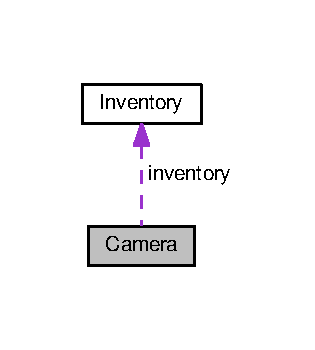
\includegraphics[width=151pt]{class_camera__coll__graph}
\end{center}
\end{figure}
\subsection*{Public Member Functions}
\begin{DoxyCompactItemize}
\item 
\hyperlink{class_camera_a01f94c3543f56ede7af49dc778f19331}{Camera} ()
\item 
void \hyperlink{class_camera_a3ab09e6714cc9b6ab58b4346b0e98011}{handle\+Movement} (S\+D\+L\+\_\+\+Event $\ast$e, S\+D\+L\+\_\+\+Window $\ast$\+\_\+window)
\item 
void \hyperlink{class_camera_a42cda7239981a5618660d04bd5893556}{update} ()
\item 
G\+Luint \hyperlink{class_camera_abab3e9c2360aa3480efc6d630e1f79e8}{get\+Place\+Type} ()
\item 
void \hyperlink{class_camera_a1f54fbe68c3810a2f4df001c671323bc}{set\+Placetype} (G\+Luint p\+T)
\end{DoxyCompactItemize}
\subsection*{Public Attributes}
\begin{DoxyCompactItemize}
\item 
glm\+::vec3 \hyperlink{class_camera_a424bcf971a87506ba6770f2c5c1073f0}{camera\+Pos}
\item 
glm\+::vec3 \hyperlink{class_camera_ad641b25d477900ac4f3cd859ac14e8f7}{camera\+Dir} = glm\+::vec3(0.\+0f, 0.\+0f, -\/1.\+0f)
\item 
glm\+::vec3 \hyperlink{class_camera_a517042b127746997f9472d51bbae2610}{camera\+Up} = glm\+::vec3(0.\+0f, 1.\+0f, 0.\+0f)
\item 
int \hyperlink{class_camera_afd43dba2d208aeb4e04dee6eb171e731}{xpos}
\item 
int \hyperlink{class_camera_a29db8762c5a7b2b9a7ffd2a31b9ffb8e}{ypos}
\item 
G\+Lfloat \hyperlink{class_camera_a2062d85e03c0fa14d5e13f3dc74c5d95}{yaw} = -\/90.\+0f
\item 
G\+Lfloat \hyperlink{class_camera_a005a78960a2726c637951b75a00925c8}{pitch} = 0.\+0f
\item 
G\+Lfloat \hyperlink{class_camera_ab551353ae0163e4483f36470d42226f2}{last\+X} = 1920/2
\item 
G\+Lfloat \hyperlink{class_camera_a3aeb91bbf0256cac3b523353795ed398}{last\+Y} = 1080/2
\item 
G\+Lfloat \hyperlink{class_camera_a8f67cd3183810d8d675d38cc62af966a}{camera\+Speed} = 1.\+0f
\item 
glm\+::mat4 \hyperlink{class_camera_add93fedd6b9a6a6e2c784aeda624de83}{view}
\item 
glm\+::mat4 \hyperlink{class_camera_a43555a0ae83f9ec696ee257e5fd48cf2}{projection}
\item 
bool \hyperlink{class_camera_aa4eb398210af281d598297d6a86c6c21}{first\+Move} = true
\item 
int \hyperlink{class_camera_a7abcf313641b6ed5be07c4c0ea04f266}{x1}
\item 
int \hyperlink{class_camera_a54e3acc8db5fb8faf8757f93bedd7a32}{y1}
\item 
glm\+::vec3 \hyperlink{class_camera_a10619630853c71114ba755595067955c}{near}
\item 
glm\+::vec3 \hyperlink{class_camera_a4188ea5916dac6f8a4edae1d0a625326}{far}
\item 
bool \hyperlink{class_camera_aba5bea2c77f7e3157307d9e272ada8ab}{mouse\+Downleft} = false
\item 
bool \hyperlink{class_camera_a3a2c6b49cdf87ea655f8d6dd97194855}{mouse\+Downright} = false
\item 
G\+Luint \hyperlink{class_camera_abcb0dd3d79e1066f6922f539b801586f}{place\+Type} = 1
\item 
\hyperlink{class_inventory}{Inventory} $\ast$ \hyperlink{class_camera_ae10beb7db168af6a6f35d4be223cccf3}{inventory}
\end{DoxyCompactItemize}


\subsection{Constructor \& Destructor Documentation}
\hypertarget{class_camera_a01f94c3543f56ede7af49dc778f19331}{}\index{Camera@{Camera}!Camera@{Camera}}
\index{Camera@{Camera}!Camera@{Camera}}
\subsubsection[{Camera}]{\setlength{\rightskip}{0pt plus 5cm}Camera\+::\+Camera (
\begin{DoxyParamCaption}
{}
\end{DoxyParamCaption}
)}\label{class_camera_a01f94c3543f56ede7af49dc778f19331}
Initialise Variables; 

\subsection{Member Function Documentation}
\hypertarget{class_camera_abab3e9c2360aa3480efc6d630e1f79e8}{}\index{Camera@{Camera}!get\+Place\+Type@{get\+Place\+Type}}
\index{get\+Place\+Type@{get\+Place\+Type}!Camera@{Camera}}
\subsubsection[{get\+Place\+Type}]{\setlength{\rightskip}{0pt plus 5cm}G\+Luint Camera\+::get\+Place\+Type (
\begin{DoxyParamCaption}
{}
\end{DoxyParamCaption}
)\hspace{0.3cm}{\ttfamily [inline]}}\label{class_camera_abab3e9c2360aa3480efc6d630e1f79e8}


Here is the caller graph for this function\+:\nopagebreak
\begin{figure}[H]
\begin{center}
\leavevmode
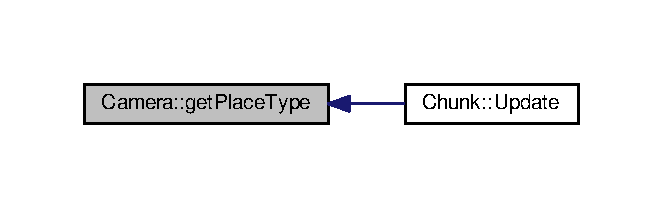
\includegraphics[width=318pt]{class_camera_abab3e9c2360aa3480efc6d630e1f79e8_icgraph}
\end{center}
\end{figure}


\hypertarget{class_camera_a3ab09e6714cc9b6ab58b4346b0e98011}{}\index{Camera@{Camera}!handle\+Movement@{handle\+Movement}}
\index{handle\+Movement@{handle\+Movement}!Camera@{Camera}}
\subsubsection[{handle\+Movement}]{\setlength{\rightskip}{0pt plus 5cm}void Camera\+::handle\+Movement (
\begin{DoxyParamCaption}
\item[{S\+D\+L\+\_\+\+Event $\ast$}]{e, }
\item[{S\+D\+L\+\_\+\+Window $\ast$}]{\+\_\+window}
\end{DoxyParamCaption}
)}\label{class_camera_a3ab09e6714cc9b6ab58b4346b0e98011}
Handle input form passed in main\+Event struct.


\begin{DoxyParams}{Parameters}
{\em S\+D\+L\+\_\+\+Event} & \\
\hline
{\em S\+D\+L\+\_\+\+Window} & \\
\hline
\end{DoxyParams}
\begin{DoxyReturn}{Returns}
N\+U\+L\+L 
\end{DoxyReturn}
Handle mouse buttons Also invert y axis to convert S\+D\+L coords to Opengl coords.

Here is the caller graph for this function\+:\nopagebreak
\begin{figure}[H]
\begin{center}
\leavevmode
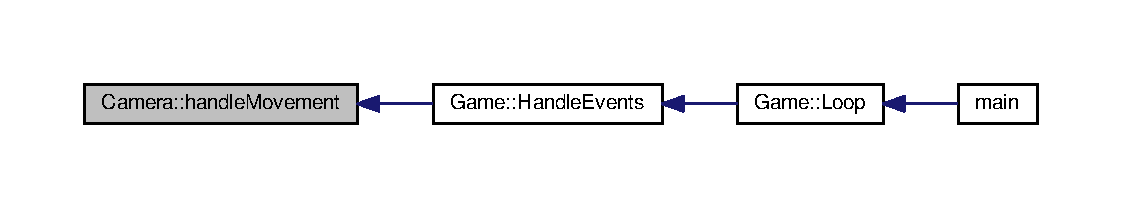
\includegraphics[width=350pt]{class_camera_a3ab09e6714cc9b6ab58b4346b0e98011_icgraph}
\end{center}
\end{figure}


\hypertarget{class_camera_a1f54fbe68c3810a2f4df001c671323bc}{}\index{Camera@{Camera}!set\+Placetype@{set\+Placetype}}
\index{set\+Placetype@{set\+Placetype}!Camera@{Camera}}
\subsubsection[{set\+Placetype}]{\setlength{\rightskip}{0pt plus 5cm}void Camera\+::set\+Placetype (
\begin{DoxyParamCaption}
\item[{G\+Luint}]{p\+T}
\end{DoxyParamCaption}
)\hspace{0.3cm}{\ttfamily [inline]}}\label{class_camera_a1f54fbe68c3810a2f4df001c671323bc}


Here is the caller graph for this function\+:\nopagebreak
\begin{figure}[H]
\begin{center}
\leavevmode
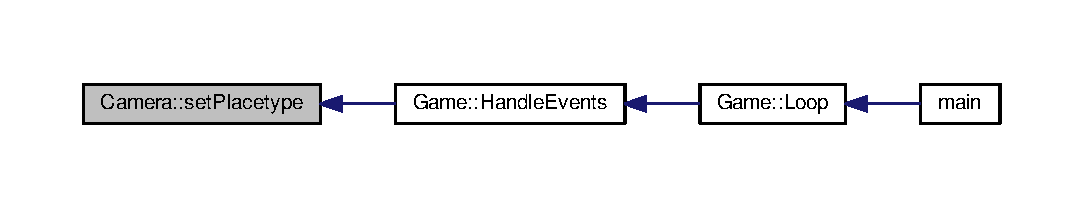
\includegraphics[width=350pt]{class_camera_a1f54fbe68c3810a2f4df001c671323bc_icgraph}
\end{center}
\end{figure}


\hypertarget{class_camera_a42cda7239981a5618660d04bd5893556}{}\index{Camera@{Camera}!update@{update}}
\index{update@{update}!Camera@{Camera}}
\subsubsection[{update}]{\setlength{\rightskip}{0pt plus 5cm}void Camera\+::update (
\begin{DoxyParamCaption}
{}
\end{DoxyParamCaption}
)}\label{class_camera_a42cda7239981a5618660d04bd5893556}
\hyperlink{class_camera}{Camera} update method.

\begin{DoxyReturn}{Returns}
N\+U\+L\+L 
\end{DoxyReturn}


Here is the caller graph for this function\+:\nopagebreak
\begin{figure}[H]
\begin{center}
\leavevmode
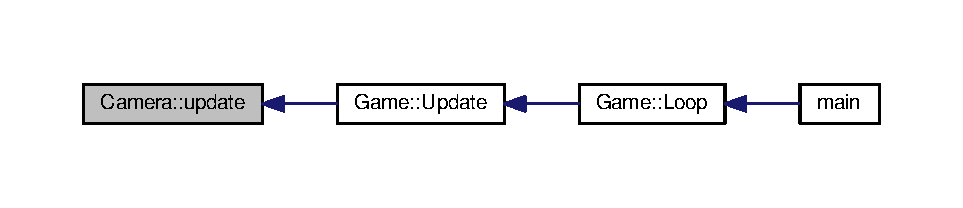
\includegraphics[width=350pt]{class_camera_a42cda7239981a5618660d04bd5893556_icgraph}
\end{center}
\end{figure}




\subsection{Member Data Documentation}
\hypertarget{class_camera_ad641b25d477900ac4f3cd859ac14e8f7}{}\index{Camera@{Camera}!camera\+Dir@{camera\+Dir}}
\index{camera\+Dir@{camera\+Dir}!Camera@{Camera}}
\subsubsection[{camera\+Dir}]{\setlength{\rightskip}{0pt plus 5cm}glm\+::vec3 Camera\+::camera\+Dir = glm\+::vec3(0.\+0f, 0.\+0f, -\/1.\+0f)}\label{class_camera_ad641b25d477900ac4f3cd859ac14e8f7}
\hypertarget{class_camera_a424bcf971a87506ba6770f2c5c1073f0}{}\index{Camera@{Camera}!camera\+Pos@{camera\+Pos}}
\index{camera\+Pos@{camera\+Pos}!Camera@{Camera}}
\subsubsection[{camera\+Pos}]{\setlength{\rightskip}{0pt plus 5cm}glm\+::vec3 Camera\+::camera\+Pos}\label{class_camera_a424bcf971a87506ba6770f2c5c1073f0}
\hypertarget{class_camera_a8f67cd3183810d8d675d38cc62af966a}{}\index{Camera@{Camera}!camera\+Speed@{camera\+Speed}}
\index{camera\+Speed@{camera\+Speed}!Camera@{Camera}}
\subsubsection[{camera\+Speed}]{\setlength{\rightskip}{0pt plus 5cm}G\+Lfloat Camera\+::camera\+Speed = 1.\+0f}\label{class_camera_a8f67cd3183810d8d675d38cc62af966a}
\hypertarget{class_camera_a517042b127746997f9472d51bbae2610}{}\index{Camera@{Camera}!camera\+Up@{camera\+Up}}
\index{camera\+Up@{camera\+Up}!Camera@{Camera}}
\subsubsection[{camera\+Up}]{\setlength{\rightskip}{0pt plus 5cm}glm\+::vec3 Camera\+::camera\+Up = glm\+::vec3(0.\+0f, 1.\+0f, 0.\+0f)}\label{class_camera_a517042b127746997f9472d51bbae2610}
\hypertarget{class_camera_a4188ea5916dac6f8a4edae1d0a625326}{}\index{Camera@{Camera}!far@{far}}
\index{far@{far}!Camera@{Camera}}
\subsubsection[{far}]{\setlength{\rightskip}{0pt plus 5cm}glm\+::vec3 Camera\+::far}\label{class_camera_a4188ea5916dac6f8a4edae1d0a625326}
\hypertarget{class_camera_aa4eb398210af281d598297d6a86c6c21}{}\index{Camera@{Camera}!first\+Move@{first\+Move}}
\index{first\+Move@{first\+Move}!Camera@{Camera}}
\subsubsection[{first\+Move}]{\setlength{\rightskip}{0pt plus 5cm}bool Camera\+::first\+Move = true}\label{class_camera_aa4eb398210af281d598297d6a86c6c21}
\hypertarget{class_camera_ae10beb7db168af6a6f35d4be223cccf3}{}\index{Camera@{Camera}!inventory@{inventory}}
\index{inventory@{inventory}!Camera@{Camera}}
\subsubsection[{inventory}]{\setlength{\rightskip}{0pt plus 5cm}{\bf Inventory}$\ast$ Camera\+::inventory}\label{class_camera_ae10beb7db168af6a6f35d4be223cccf3}
\hypertarget{class_camera_ab551353ae0163e4483f36470d42226f2}{}\index{Camera@{Camera}!last\+X@{last\+X}}
\index{last\+X@{last\+X}!Camera@{Camera}}
\subsubsection[{last\+X}]{\setlength{\rightskip}{0pt plus 5cm}G\+Lfloat Camera\+::last\+X = 1920/2}\label{class_camera_ab551353ae0163e4483f36470d42226f2}
\hypertarget{class_camera_a3aeb91bbf0256cac3b523353795ed398}{}\index{Camera@{Camera}!last\+Y@{last\+Y}}
\index{last\+Y@{last\+Y}!Camera@{Camera}}
\subsubsection[{last\+Y}]{\setlength{\rightskip}{0pt plus 5cm}G\+Lfloat Camera\+::last\+Y = 1080/2}\label{class_camera_a3aeb91bbf0256cac3b523353795ed398}
\hypertarget{class_camera_aba5bea2c77f7e3157307d9e272ada8ab}{}\index{Camera@{Camera}!mouse\+Downleft@{mouse\+Downleft}}
\index{mouse\+Downleft@{mouse\+Downleft}!Camera@{Camera}}
\subsubsection[{mouse\+Downleft}]{\setlength{\rightskip}{0pt plus 5cm}bool Camera\+::mouse\+Downleft = false}\label{class_camera_aba5bea2c77f7e3157307d9e272ada8ab}
\hypertarget{class_camera_a3a2c6b49cdf87ea655f8d6dd97194855}{}\index{Camera@{Camera}!mouse\+Downright@{mouse\+Downright}}
\index{mouse\+Downright@{mouse\+Downright}!Camera@{Camera}}
\subsubsection[{mouse\+Downright}]{\setlength{\rightskip}{0pt plus 5cm}bool Camera\+::mouse\+Downright = false}\label{class_camera_a3a2c6b49cdf87ea655f8d6dd97194855}
\hypertarget{class_camera_a10619630853c71114ba755595067955c}{}\index{Camera@{Camera}!near@{near}}
\index{near@{near}!Camera@{Camera}}
\subsubsection[{near}]{\setlength{\rightskip}{0pt plus 5cm}glm\+::vec3 Camera\+::near}\label{class_camera_a10619630853c71114ba755595067955c}
\hypertarget{class_camera_a005a78960a2726c637951b75a00925c8}{}\index{Camera@{Camera}!pitch@{pitch}}
\index{pitch@{pitch}!Camera@{Camera}}
\subsubsection[{pitch}]{\setlength{\rightskip}{0pt plus 5cm}G\+Lfloat Camera\+::pitch = 0.\+0f}\label{class_camera_a005a78960a2726c637951b75a00925c8}
\hypertarget{class_camera_abcb0dd3d79e1066f6922f539b801586f}{}\index{Camera@{Camera}!place\+Type@{place\+Type}}
\index{place\+Type@{place\+Type}!Camera@{Camera}}
\subsubsection[{place\+Type}]{\setlength{\rightskip}{0pt plus 5cm}G\+Luint Camera\+::place\+Type = 1}\label{class_camera_abcb0dd3d79e1066f6922f539b801586f}
\hypertarget{class_camera_a43555a0ae83f9ec696ee257e5fd48cf2}{}\index{Camera@{Camera}!projection@{projection}}
\index{projection@{projection}!Camera@{Camera}}
\subsubsection[{projection}]{\setlength{\rightskip}{0pt plus 5cm}glm\+::mat4 Camera\+::projection}\label{class_camera_a43555a0ae83f9ec696ee257e5fd48cf2}
\hypertarget{class_camera_add93fedd6b9a6a6e2c784aeda624de83}{}\index{Camera@{Camera}!view@{view}}
\index{view@{view}!Camera@{Camera}}
\subsubsection[{view}]{\setlength{\rightskip}{0pt plus 5cm}glm\+::mat4 Camera\+::view}\label{class_camera_add93fedd6b9a6a6e2c784aeda624de83}
\hypertarget{class_camera_a7abcf313641b6ed5be07c4c0ea04f266}{}\index{Camera@{Camera}!x1@{x1}}
\index{x1@{x1}!Camera@{Camera}}
\subsubsection[{x1}]{\setlength{\rightskip}{0pt plus 5cm}int Camera\+::x1}\label{class_camera_a7abcf313641b6ed5be07c4c0ea04f266}
\hypertarget{class_camera_afd43dba2d208aeb4e04dee6eb171e731}{}\index{Camera@{Camera}!xpos@{xpos}}
\index{xpos@{xpos}!Camera@{Camera}}
\subsubsection[{xpos}]{\setlength{\rightskip}{0pt plus 5cm}int Camera\+::xpos}\label{class_camera_afd43dba2d208aeb4e04dee6eb171e731}
\hypertarget{class_camera_a54e3acc8db5fb8faf8757f93bedd7a32}{}\index{Camera@{Camera}!y1@{y1}}
\index{y1@{y1}!Camera@{Camera}}
\subsubsection[{y1}]{\setlength{\rightskip}{0pt plus 5cm}int Camera\+::y1}\label{class_camera_a54e3acc8db5fb8faf8757f93bedd7a32}
\hypertarget{class_camera_a2062d85e03c0fa14d5e13f3dc74c5d95}{}\index{Camera@{Camera}!yaw@{yaw}}
\index{yaw@{yaw}!Camera@{Camera}}
\subsubsection[{yaw}]{\setlength{\rightskip}{0pt plus 5cm}G\+Lfloat Camera\+::yaw = -\/90.\+0f}\label{class_camera_a2062d85e03c0fa14d5e13f3dc74c5d95}
\hypertarget{class_camera_a29db8762c5a7b2b9a7ffd2a31b9ffb8e}{}\index{Camera@{Camera}!ypos@{ypos}}
\index{ypos@{ypos}!Camera@{Camera}}
\subsubsection[{ypos}]{\setlength{\rightskip}{0pt plus 5cm}int Camera\+::ypos}\label{class_camera_a29db8762c5a7b2b9a7ffd2a31b9ffb8e}


The documentation for this class was generated from the following files\+:\begin{DoxyCompactItemize}
\item 
src/\hyperlink{_camera_8h}{Camera.\+h}\item 
src/\hyperlink{_camera_8cpp}{Camera.\+cpp}\end{DoxyCompactItemize}

\hypertarget{class_chunk}{}\section{Chunk Class Reference}
\label{class_chunk}\index{Chunk@{Chunk}}


{\ttfamily \#include $<$Chunk.\+h$>$}

\subsection*{Public Member Functions}
\begin{DoxyCompactItemize}
\item 
\hyperlink{class_chunk_acc32e1562cad6664c98ee07edecdbdf9}{Chunk} ()
\item 
\hyperlink{class_chunk_a83076c5f08f43296f3d6fb39c406b68f}{Chunk} (G\+Lfloat X, G\+Lfloat Y, G\+Lfloat Z, \hyperlink{class_perlin}{Perlin} noise)
\item 
\hyperlink{class_chunk_ad21b515f41c9a1d21740b9e7e3f8eede}{$\sim$\+Chunk} ()
\item 
void \hyperlink{class_chunk_a6e993f948335d6ead2ec2eee206af847}{Update} (\hyperlink{class_camera}{Camera} $\ast$camera)
\item 
void \hyperlink{class_chunk_a3c85fe052765b8c1da975b1f7fc60637}{Render} (\hyperlink{class_shader}{Shader} shader, \hyperlink{class_camera}{Camera} $\ast$camera)
\item 
void \hyperlink{class_chunk_ae50a8df55381d68288831e392012a938}{Init} ()
\end{DoxyCompactItemize}


\subsection{Constructor \& Destructor Documentation}
\hypertarget{class_chunk_acc32e1562cad6664c98ee07edecdbdf9}{}\index{Chunk@{Chunk}!Chunk@{Chunk}}
\index{Chunk@{Chunk}!Chunk@{Chunk}}
\subsubsection[{Chunk}]{\setlength{\rightskip}{0pt plus 5cm}Chunk\+::\+Chunk (
\begin{DoxyParamCaption}
{}
\end{DoxyParamCaption}
)}\label{class_chunk_acc32e1562cad6664c98ee07edecdbdf9}
\hyperlink{class_chunk}{Chunk} constructor initialises values to zero. 

Here is the call graph for this function\+:
\nopagebreak
\begin{figure}[H]
\begin{center}
\leavevmode
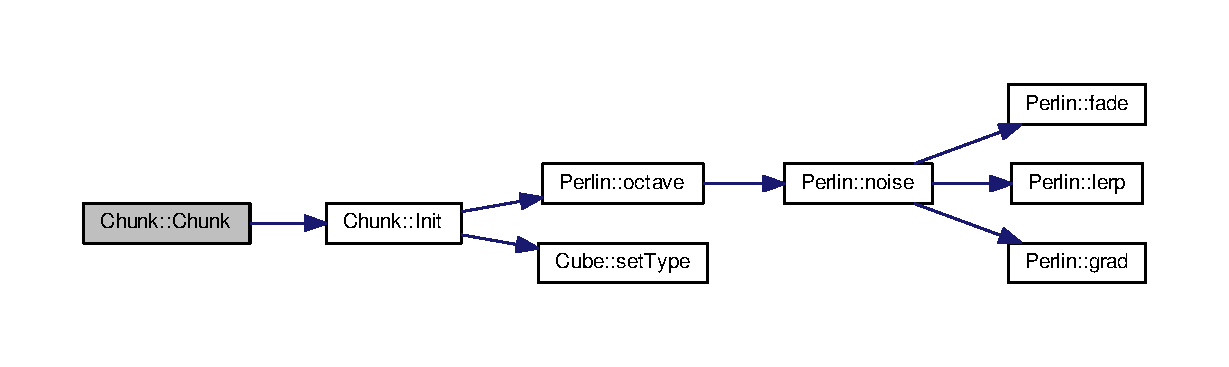
\includegraphics[width=350pt]{class_chunk_acc32e1562cad6664c98ee07edecdbdf9_cgraph}
\end{center}
\end{figure}


\hypertarget{class_chunk_a83076c5f08f43296f3d6fb39c406b68f}{}\index{Chunk@{Chunk}!Chunk@{Chunk}}
\index{Chunk@{Chunk}!Chunk@{Chunk}}
\subsubsection[{Chunk}]{\setlength{\rightskip}{0pt plus 5cm}Chunk\+::\+Chunk (
\begin{DoxyParamCaption}
\item[{G\+Lfloat}]{X, }
\item[{G\+Lfloat}]{Y, }
\item[{G\+Lfloat}]{Z, }
\item[{{\bf Perlin}}]{noise}
\end{DoxyParamCaption}
)}\label{class_chunk_a83076c5f08f43296f3d6fb39c406b68f}
Overloaded \hyperlink{class_chunk}{Chunk} constructor that sets the position and noise used to generate the chunk.


\begin{DoxyParams}{Parameters}
{\em X} & -\/ x position of the chunk \\
\hline
{\em Y} & -\/ y position of the chunk \\
\hline
{\em Z} & -\/ z position of the chunk \\
\hline
{\em noise} & -\/ the P\+Erlin noise being used to generate this chunk.\\
\hline
\end{DoxyParams}
\begin{DoxyReturn}{Returns}
N\+U\+L\+L 
\end{DoxyReturn}


Here is the call graph for this function\+:
\nopagebreak
\begin{figure}[H]
\begin{center}
\leavevmode
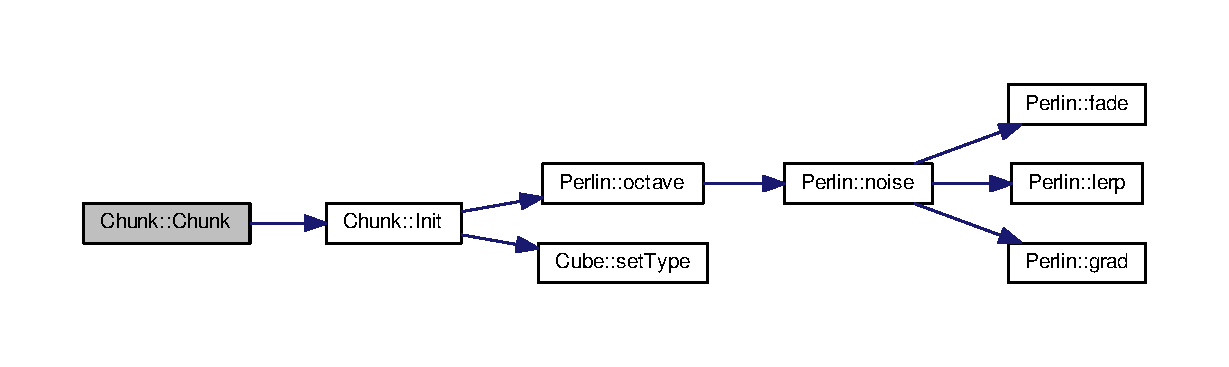
\includegraphics[width=350pt]{class_chunk_a83076c5f08f43296f3d6fb39c406b68f_cgraph}
\end{center}
\end{figure}


\hypertarget{class_chunk_ad21b515f41c9a1d21740b9e7e3f8eede}{}\index{Chunk@{Chunk}!````~Chunk@{$\sim$\+Chunk}}
\index{````~Chunk@{$\sim$\+Chunk}!Chunk@{Chunk}}
\subsubsection[{$\sim$\+Chunk}]{\setlength{\rightskip}{0pt plus 5cm}Chunk\+::$\sim$\+Chunk (
\begin{DoxyParamCaption}
{}
\end{DoxyParamCaption}
)}\label{class_chunk_ad21b515f41c9a1d21740b9e7e3f8eede}
\hyperlink{class_chunk}{Chunk} destructor. 

\subsection{Member Function Documentation}
\hypertarget{class_chunk_ae50a8df55381d68288831e392012a938}{}\index{Chunk@{Chunk}!Init@{Init}}
\index{Init@{Init}!Chunk@{Chunk}}
\subsubsection[{Init}]{\setlength{\rightskip}{0pt plus 5cm}void Chunk\+::\+Init (
\begin{DoxyParamCaption}
{}
\end{DoxyParamCaption}
)}\label{class_chunk_ae50a8df55381d68288831e392012a938}
\hyperlink{class_chunk}{Chunk} initialisation method. Sets up the chunks model from the perlin noise passed into the constructor.

\begin{DoxyReturn}{Returns}
N\+U\+L\+L 
\end{DoxyReturn}


Here is the call graph for this function\+:
\nopagebreak
\begin{figure}[H]
\begin{center}
\leavevmode
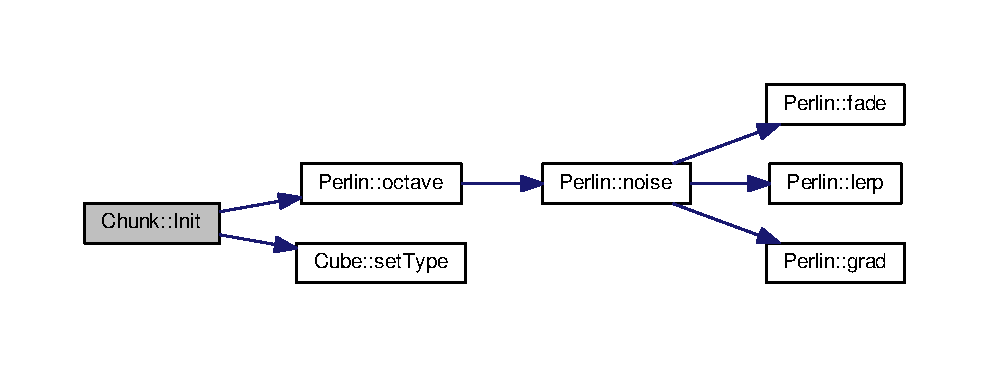
\includegraphics[width=350pt]{class_chunk_ae50a8df55381d68288831e392012a938_cgraph}
\end{center}
\end{figure}




Here is the caller graph for this function\+:\nopagebreak
\begin{figure}[H]
\begin{center}
\leavevmode
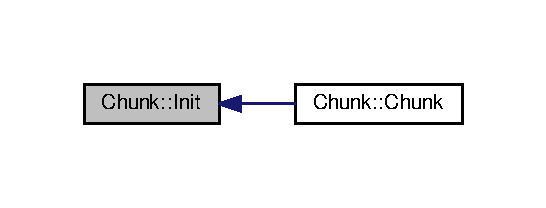
\includegraphics[width=262pt]{class_chunk_ae50a8df55381d68288831e392012a938_icgraph}
\end{center}
\end{figure}


\hypertarget{class_chunk_a3c85fe052765b8c1da975b1f7fc60637}{}\index{Chunk@{Chunk}!Render@{Render}}
\index{Render@{Render}!Chunk@{Chunk}}
\subsubsection[{Render}]{\setlength{\rightskip}{0pt plus 5cm}void Chunk\+::\+Render (
\begin{DoxyParamCaption}
\item[{{\bf Shader}}]{shader, }
\item[{{\bf Camera} $\ast$}]{camera}
\end{DoxyParamCaption}
)}\label{class_chunk_a3c85fe052765b8c1da975b1f7fc60637}
Chunks render function.


\begin{DoxyParams}{Parameters}
{\em shader} & -\/ The shader being used to render the cubes gets passed to the cubes when there render function is called. \\
\hline
{\em camera} & -\/ The camera that will see the rendered chunks.\\
\hline
\end{DoxyParams}
\begin{DoxyReturn}{Returns}
N\+U\+L\+L 
\end{DoxyReturn}
If one of 6 neighbours is air. This way if a face is visible the cube is rendered.

Here is the call graph for this function\+:\nopagebreak
\begin{figure}[H]
\begin{center}
\leavevmode
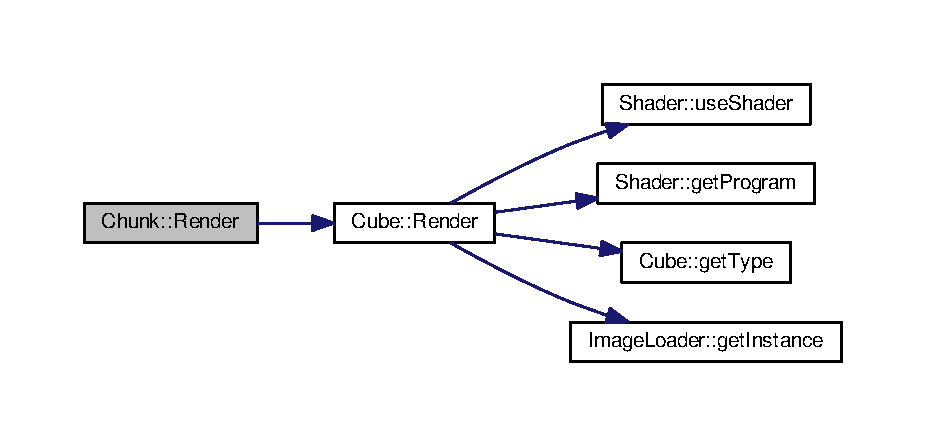
\includegraphics[width=350pt]{class_chunk_a3c85fe052765b8c1da975b1f7fc60637_cgraph}
\end{center}
\end{figure}


\hypertarget{class_chunk_a6e993f948335d6ead2ec2eee206af847}{}\index{Chunk@{Chunk}!Update@{Update}}
\index{Update@{Update}!Chunk@{Chunk}}
\subsubsection[{Update}]{\setlength{\rightskip}{0pt plus 5cm}void Chunk\+::\+Update (
\begin{DoxyParamCaption}
\item[{{\bf Camera} $\ast$}]{cam}
\end{DoxyParamCaption}
)}\label{class_chunk_a6e993f948335d6ead2ec2eee206af847}
Chunks update method.


\begin{DoxyParams}{Parameters}
{\em cam} & -\/ the camera that will be used to test for collisions with cubes when it moves.\\
\hline
\end{DoxyParams}
\begin{DoxyReturn}{Returns}
N\+U\+L\+L 
\end{DoxyReturn}


Here is the call graph for this function\+:\nopagebreak
\begin{figure}[H]
\begin{center}
\leavevmode
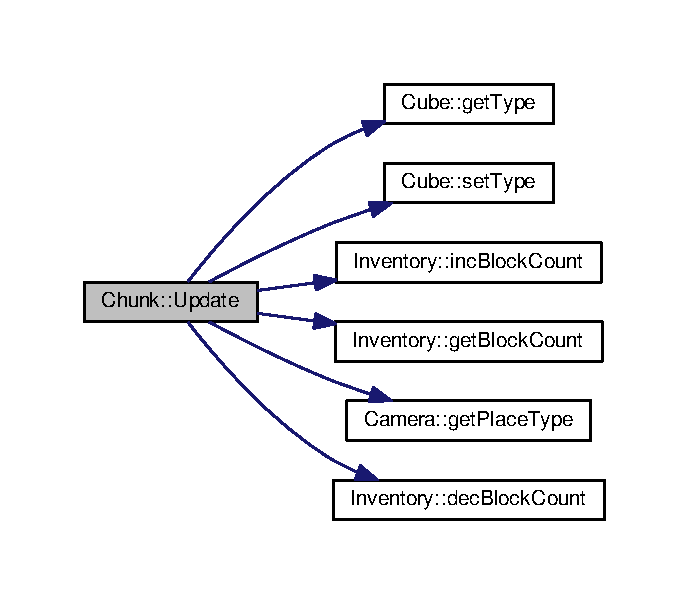
\includegraphics[width=330pt]{class_chunk_a6e993f948335d6ead2ec2eee206af847_cgraph}
\end{center}
\end{figure}




The documentation for this class was generated from the following files\+:\begin{DoxyCompactItemize}
\item 
src/\hyperlink{_chunk_8h}{Chunk.\+h}\item 
src/\hyperlink{_chunk_8cpp}{Chunk.\+cpp}\end{DoxyCompactItemize}

\hypertarget{class_cube}{}\section{Cube Class Reference}
\label{class_cube}\index{Cube@{Cube}}


{\ttfamily \#include $<$Cube.\+h$>$}

\subsection*{Public Types}
\begin{DoxyCompactItemize}
\item 
enum \hyperlink{class_cube_aa23329b4c4998aa957e44b6a44b9bfcf}{Type} \{ \hyperlink{class_cube_aa23329b4c4998aa957e44b6a44b9bfcfa96d073bf026e7fda861a7abe6b06df48}{Air} = 0, 
\hyperlink{class_cube_aa23329b4c4998aa957e44b6a44b9bfcfa39debf286eddf291013f7956e2e241ce}{Dirt} = 1, 
\hyperlink{class_cube_aa23329b4c4998aa957e44b6a44b9bfcfad77c682c3ef00d11319a1bed70ff9556}{Stone} = 2
 \}
\end{DoxyCompactItemize}
\subsection*{Public Member Functions}
\begin{DoxyCompactItemize}
\item 
\hyperlink{class_cube_a06f3d86fb63e3aad08623610aa3c17b4}{Cube} ()
\item 
\hyperlink{class_cube_a8523687590ff90c49bc54281d0d3e47a}{Cube} (G\+Lfloat x, G\+Lfloat y, G\+Lfloat z)
\item 
\hyperlink{class_cube_aa814e979cecb8c451fdb332ded2cea1e}{$\sim$\+Cube} ()
\item 
glm\+::vec3 \hyperlink{class_cube_ae55713af649b1cc24426d2ca209b8163}{get\+Position} ()
\item 
void \hyperlink{class_cube_a6940368c7d15292b4bccdf3ffc67ec93}{set\+Position} (G\+Lfloat x, G\+Lfloat y, G\+Lfloat z)
\item 
void \hyperlink{class_cube_aeeeccb9eb5da6e9d8114be298742cf00}{Render} (\hyperlink{class_shader}{Shader} shader, \hyperlink{class_camera}{Camera} $\ast$camera)
\item 
G\+Luint \hyperlink{class_cube_a92ef19e9427e3d4f098d575db03757c6}{get\+Texture} ()
\item 
void \hyperlink{class_cube_a13e5899692dffbb09019809d2998f71a}{load\+Cube} ()
\item 
G\+Luint \hyperlink{class_cube_af4f3394054081c69c8f4f9c2a6b9ba54}{get\+V\+A\+O} ()
\item 
G\+Luint \hyperlink{class_cube_aec756e9d5ff559a226ce52a300688508}{get\+V\+B\+O} ()
\item 
void \hyperlink{class_cube_ab68cedd92c926506f50f06ae57761ae7}{set\+Type} (G\+Luint cube\+Type)
\item 
G\+Luint \hyperlink{class_cube_a27aea823ea0926b6fb9315ae9cfac5bb}{get\+Type} ()
\end{DoxyCompactItemize}


\subsection{Member Enumeration Documentation}
\hypertarget{class_cube_aa23329b4c4998aa957e44b6a44b9bfcf}{}\index{Cube@{Cube}!Type@{Type}}
\index{Type@{Type}!Cube@{Cube}}
\subsubsection[{Type}]{\setlength{\rightskip}{0pt plus 5cm}enum {\bf Cube\+::\+Type}}\label{class_cube_aa23329b4c4998aa957e44b6a44b9bfcf}
\begin{Desc}
\item[Enumerator]\par
\begin{description}
\index{Air@{Air}!Cube@{Cube}}\index{Cube@{Cube}!Air@{Air}}\item[{\em 
\hypertarget{class_cube_aa23329b4c4998aa957e44b6a44b9bfcfa96d073bf026e7fda861a7abe6b06df48}{}Air\label{class_cube_aa23329b4c4998aa957e44b6a44b9bfcfa96d073bf026e7fda861a7abe6b06df48}
}]\index{Dirt@{Dirt}!Cube@{Cube}}\index{Cube@{Cube}!Dirt@{Dirt}}\item[{\em 
\hypertarget{class_cube_aa23329b4c4998aa957e44b6a44b9bfcfa39debf286eddf291013f7956e2e241ce}{}Dirt\label{class_cube_aa23329b4c4998aa957e44b6a44b9bfcfa39debf286eddf291013f7956e2e241ce}
}]\index{Stone@{Stone}!Cube@{Cube}}\index{Cube@{Cube}!Stone@{Stone}}\item[{\em 
\hypertarget{class_cube_aa23329b4c4998aa957e44b6a44b9bfcfad77c682c3ef00d11319a1bed70ff9556}{}Stone\label{class_cube_aa23329b4c4998aa957e44b6a44b9bfcfad77c682c3ef00d11319a1bed70ff9556}
}]\end{description}
\end{Desc}


\subsection{Constructor \& Destructor Documentation}
\hypertarget{class_cube_a06f3d86fb63e3aad08623610aa3c17b4}{}\index{Cube@{Cube}!Cube@{Cube}}
\index{Cube@{Cube}!Cube@{Cube}}
\subsubsection[{Cube}]{\setlength{\rightskip}{0pt plus 5cm}Cube\+::\+Cube (
\begin{DoxyParamCaption}
{}
\end{DoxyParamCaption}
)}\label{class_cube_a06f3d86fb63e3aad08623610aa3c17b4}
Default \hyperlink{class_cube}{Cube} constructor 

Here is the call graph for this function\+:\nopagebreak
\begin{figure}[H]
\begin{center}
\leavevmode
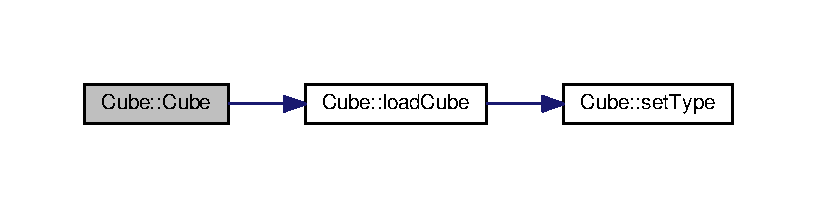
\includegraphics[width=350pt]{class_cube_a06f3d86fb63e3aad08623610aa3c17b4_cgraph}
\end{center}
\end{figure}


\hypertarget{class_cube_a8523687590ff90c49bc54281d0d3e47a}{}\index{Cube@{Cube}!Cube@{Cube}}
\index{Cube@{Cube}!Cube@{Cube}}
\subsubsection[{Cube}]{\setlength{\rightskip}{0pt plus 5cm}Cube\+::\+Cube (
\begin{DoxyParamCaption}
\item[{G\+Lfloat}]{x, }
\item[{G\+Lfloat}]{y, }
\item[{G\+Lfloat}]{z}
\end{DoxyParamCaption}
)}\label{class_cube_a8523687590ff90c49bc54281d0d3e47a}
Overload \hyperlink{class_cube}{Cube} constructor


\begin{DoxyParams}{Parameters}
{\em G\+Lfloat} & x , y , z \\
\hline
\end{DoxyParams}


Here is the call graph for this function\+:\nopagebreak
\begin{figure}[H]
\begin{center}
\leavevmode
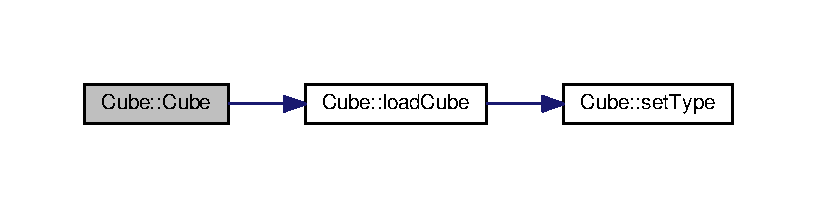
\includegraphics[width=350pt]{class_cube_a8523687590ff90c49bc54281d0d3e47a_cgraph}
\end{center}
\end{figure}


\hypertarget{class_cube_aa814e979cecb8c451fdb332ded2cea1e}{}\index{Cube@{Cube}!````~Cube@{$\sim$\+Cube}}
\index{````~Cube@{$\sim$\+Cube}!Cube@{Cube}}
\subsubsection[{$\sim$\+Cube}]{\setlength{\rightskip}{0pt plus 5cm}Cube\+::$\sim$\+Cube (
\begin{DoxyParamCaption}
{}
\end{DoxyParamCaption}
)}\label{class_cube_aa814e979cecb8c451fdb332ded2cea1e}


\subsection{Member Function Documentation}
\hypertarget{class_cube_ae55713af649b1cc24426d2ca209b8163}{}\index{Cube@{Cube}!get\+Position@{get\+Position}}
\index{get\+Position@{get\+Position}!Cube@{Cube}}
\subsubsection[{get\+Position}]{\setlength{\rightskip}{0pt plus 5cm}glm\+::vec3 Cube\+::get\+Position (
\begin{DoxyParamCaption}
{}
\end{DoxyParamCaption}
)}\label{class_cube_ae55713af649b1cc24426d2ca209b8163}
Get method for position

\begin{DoxyReturn}{Returns}
glm\+::vec3 
\end{DoxyReturn}
\hypertarget{class_cube_a92ef19e9427e3d4f098d575db03757c6}{}\index{Cube@{Cube}!get\+Texture@{get\+Texture}}
\index{get\+Texture@{get\+Texture}!Cube@{Cube}}
\subsubsection[{get\+Texture}]{\setlength{\rightskip}{0pt plus 5cm}G\+Luint Cube\+::get\+Texture (
\begin{DoxyParamCaption}
{}
\end{DoxyParamCaption}
)}\label{class_cube_a92ef19e9427e3d4f098d575db03757c6}
Get method for texture

\begin{DoxyReturn}{Returns}
G\+Luint 
\end{DoxyReturn}
\hypertarget{class_cube_a27aea823ea0926b6fb9315ae9cfac5bb}{}\index{Cube@{Cube}!get\+Type@{get\+Type}}
\index{get\+Type@{get\+Type}!Cube@{Cube}}
\subsubsection[{get\+Type}]{\setlength{\rightskip}{0pt plus 5cm}G\+Luint Cube\+::get\+Type (
\begin{DoxyParamCaption}
{}
\end{DoxyParamCaption}
)}\label{class_cube_a27aea823ea0926b6fb9315ae9cfac5bb}
Get method for type

\begin{DoxyReturn}{Returns}
N\+U\+L\+L 
\end{DoxyReturn}


Here is the caller graph for this function\+:\nopagebreak
\begin{figure}[H]
\begin{center}
\leavevmode
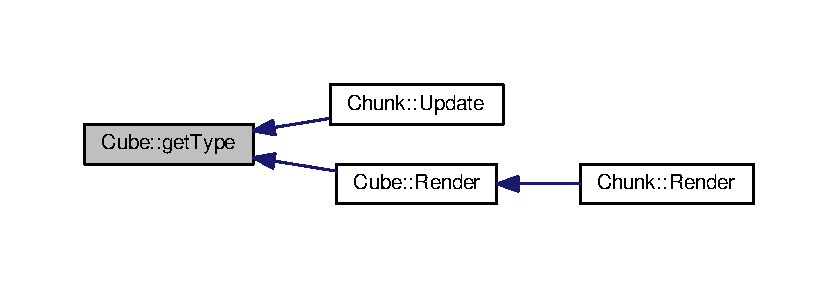
\includegraphics[width=350pt]{class_cube_a27aea823ea0926b6fb9315ae9cfac5bb_icgraph}
\end{center}
\end{figure}


\hypertarget{class_cube_af4f3394054081c69c8f4f9c2a6b9ba54}{}\index{Cube@{Cube}!get\+V\+A\+O@{get\+V\+A\+O}}
\index{get\+V\+A\+O@{get\+V\+A\+O}!Cube@{Cube}}
\subsubsection[{get\+V\+A\+O}]{\setlength{\rightskip}{0pt plus 5cm}G\+Luint Cube\+::get\+V\+A\+O (
\begin{DoxyParamCaption}
{}
\end{DoxyParamCaption}
)}\label{class_cube_af4f3394054081c69c8f4f9c2a6b9ba54}
Get method for vertex array object

\begin{DoxyReturn}{Returns}
G\+Luint 
\end{DoxyReturn}
\hypertarget{class_cube_aec756e9d5ff559a226ce52a300688508}{}\index{Cube@{Cube}!get\+V\+B\+O@{get\+V\+B\+O}}
\index{get\+V\+B\+O@{get\+V\+B\+O}!Cube@{Cube}}
\subsubsection[{get\+V\+B\+O}]{\setlength{\rightskip}{0pt plus 5cm}G\+Luint Cube\+::get\+V\+B\+O (
\begin{DoxyParamCaption}
{}
\end{DoxyParamCaption}
)}\label{class_cube_aec756e9d5ff559a226ce52a300688508}
Get method for vertex buffer object

\begin{DoxyReturn}{Returns}
G\+Luint 
\end{DoxyReturn}
\hypertarget{class_cube_a13e5899692dffbb09019809d2998f71a}{}\index{Cube@{Cube}!load\+Cube@{load\+Cube}}
\index{load\+Cube@{load\+Cube}!Cube@{Cube}}
\subsubsection[{load\+Cube}]{\setlength{\rightskip}{0pt plus 5cm}void Cube\+::load\+Cube (
\begin{DoxyParamCaption}
{}
\end{DoxyParamCaption}
)}\label{class_cube_a13e5899692dffbb09019809d2998f71a}
load cube to grpahics memory

\begin{DoxyReturn}{Returns}
N\+U\+L\+L 
\end{DoxyReturn}


Here is the call graph for this function\+:\nopagebreak
\begin{figure}[H]
\begin{center}
\leavevmode
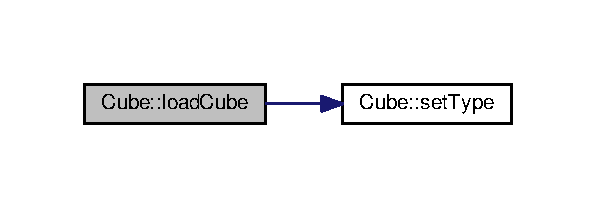
\includegraphics[width=286pt]{class_cube_a13e5899692dffbb09019809d2998f71a_cgraph}
\end{center}
\end{figure}




Here is the caller graph for this function\+:\nopagebreak
\begin{figure}[H]
\begin{center}
\leavevmode
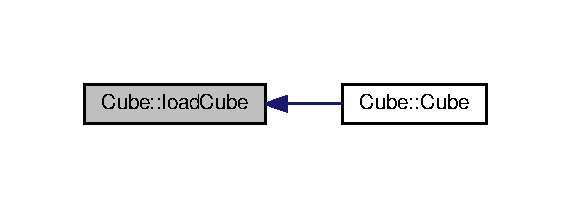
\includegraphics[width=274pt]{class_cube_a13e5899692dffbb09019809d2998f71a_icgraph}
\end{center}
\end{figure}


\hypertarget{class_cube_aeeeccb9eb5da6e9d8114be298742cf00}{}\index{Cube@{Cube}!Render@{Render}}
\index{Render@{Render}!Cube@{Cube}}
\subsubsection[{Render}]{\setlength{\rightskip}{0pt plus 5cm}void Cube\+::\+Render (
\begin{DoxyParamCaption}
\item[{{\bf Shader}}]{shader, }
\item[{{\bf Camera} $\ast$}]{camera}
\end{DoxyParamCaption}
)}\label{class_cube_aeeeccb9eb5da6e9d8114be298742cf00}
Render method


\begin{DoxyParams}{Parameters}
{\em \hyperlink{class_shader}{Shader}} & \\
\hline
{\em \hyperlink{class_camera}{Camera}} & \\
\hline
\end{DoxyParams}
\begin{DoxyReturn}{Returns}
N\+U\+L\+L 
\end{DoxyReturn}


Here is the call graph for this function\+:\nopagebreak
\begin{figure}[H]
\begin{center}
\leavevmode
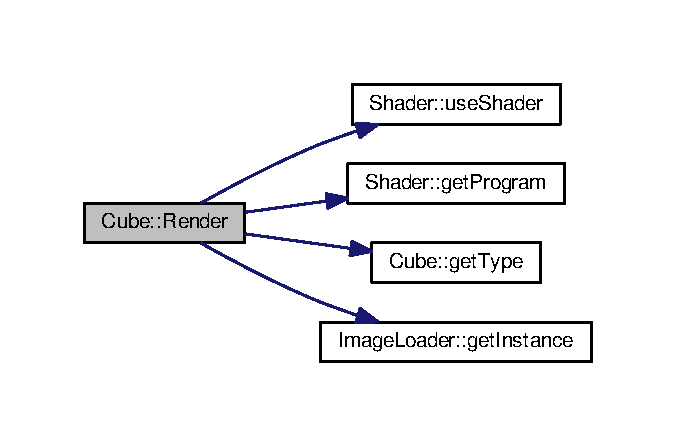
\includegraphics[width=324pt]{class_cube_aeeeccb9eb5da6e9d8114be298742cf00_cgraph}
\end{center}
\end{figure}




Here is the caller graph for this function\+:\nopagebreak
\begin{figure}[H]
\begin{center}
\leavevmode
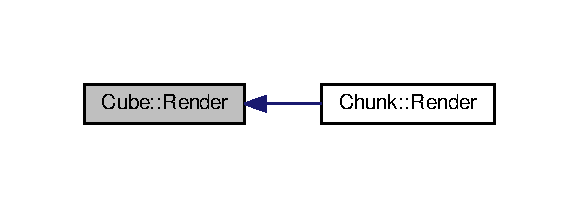
\includegraphics[width=278pt]{class_cube_aeeeccb9eb5da6e9d8114be298742cf00_icgraph}
\end{center}
\end{figure}


\hypertarget{class_cube_a6940368c7d15292b4bccdf3ffc67ec93}{}\index{Cube@{Cube}!set\+Position@{set\+Position}}
\index{set\+Position@{set\+Position}!Cube@{Cube}}
\subsubsection[{set\+Position}]{\setlength{\rightskip}{0pt plus 5cm}void Cube\+::set\+Position (
\begin{DoxyParamCaption}
\item[{G\+Lfloat}]{x, }
\item[{G\+Lfloat}]{y, }
\item[{G\+Lfloat}]{z}
\end{DoxyParamCaption}
)}\label{class_cube_a6940368c7d15292b4bccdf3ffc67ec93}
Set method for position


\begin{DoxyParams}{Parameters}
{\em G\+Lfloat} & x , y, , z\\
\hline
\end{DoxyParams}
\begin{DoxyReturn}{Returns}
N\+U\+L\+L 
\end{DoxyReturn}
\hypertarget{class_cube_ab68cedd92c926506f50f06ae57761ae7}{}\index{Cube@{Cube}!set\+Type@{set\+Type}}
\index{set\+Type@{set\+Type}!Cube@{Cube}}
\subsubsection[{set\+Type}]{\setlength{\rightskip}{0pt plus 5cm}void Cube\+::set\+Type (
\begin{DoxyParamCaption}
\item[{G\+Luint}]{cube\+Type}
\end{DoxyParamCaption}
)}\label{class_cube_ab68cedd92c926506f50f06ae57761ae7}
Set method for type

\begin{DoxyReturn}{Returns}
G\+Luint 
\end{DoxyReturn}


Here is the caller graph for this function\+:\nopagebreak
\begin{figure}[H]
\begin{center}
\leavevmode
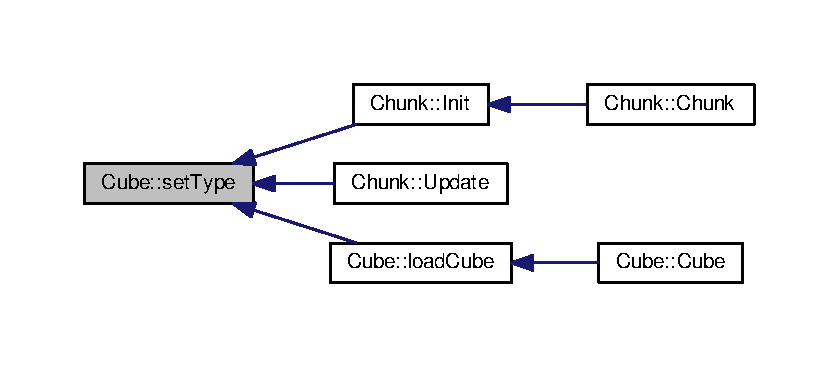
\includegraphics[width=350pt]{class_cube_ab68cedd92c926506f50f06ae57761ae7_icgraph}
\end{center}
\end{figure}




The documentation for this class was generated from the following files\+:\begin{DoxyCompactItemize}
\item 
src/\hyperlink{_cube_8h}{Cube.\+h}\item 
src/\hyperlink{_cube_8cpp}{Cube.\+cpp}\end{DoxyCompactItemize}

\hypertarget{class_game}{}\section{Game Class Reference}
\label{class_game}\index{Game@{Game}}


{\ttfamily \#include $<$Game.\+h$>$}

\subsection*{Public Member Functions}
\begin{DoxyCompactItemize}
\item 
\hyperlink{class_game_ad59df6562a58a614fda24622d3715b65}{Game} ()
\item 
\hyperlink{class_game_ae3d112ca6e0e55150d2fdbc704474530}{$\sim$\+Game} ()
\item 
void \hyperlink{class_game_a555a9e4719fd49971765a2ab8b090b5c}{Init} ()
\item 
void \hyperlink{class_game_a28d8a0a65bda89be42d9c46fc2e4f14b}{Loop} ()
\item 
void \hyperlink{class_game_afe8f2a4980f240bbfba8c1f495ff5075}{Clean\+Up} ()
\item 
void \hyperlink{class_game_a0897730fc9fed789f6c0f11d21a0c14a}{Render} ()
\item 
void \hyperlink{class_game_a1c5373c68261c54aff03e6abe40fee52}{Update} ()
\item 
void \hyperlink{class_game_a6b7a69223477dbfae5f570763385a2f1}{Handle\+Events} (S\+D\+L\+\_\+\+Event e, S\+D\+L\+\_\+\+Window $\ast$\hyperlink{class_game_ac93b435b5da2f81e01da94a2871c1394}{\+\_\+window})
\item 
void \hyperlink{class_game_a7b9c3ffde53cdf3fa685d6e9b5ae43f3}{objinit} ()
\end{DoxyCompactItemize}
\subsection*{Public Attributes}
\begin{DoxyCompactItemize}
\item 
S\+D\+L\+\_\+\+Window $\ast$ \hyperlink{class_game_ac93b435b5da2f81e01da94a2871c1394}{\+\_\+window}
\end{DoxyCompactItemize}


\subsection{Constructor \& Destructor Documentation}
\hypertarget{class_game_ad59df6562a58a614fda24622d3715b65}{}\index{Game@{Game}!Game@{Game}}
\index{Game@{Game}!Game@{Game}}
\subsubsection[{Game}]{\setlength{\rightskip}{0pt plus 5cm}Game\+::\+Game (
\begin{DoxyParamCaption}
{}
\end{DoxyParamCaption}
)}\label{class_game_ad59df6562a58a614fda24622d3715b65}
\hypertarget{class_game_ae3d112ca6e0e55150d2fdbc704474530}{}\index{Game@{Game}!````~Game@{$\sim$\+Game}}
\index{````~Game@{$\sim$\+Game}!Game@{Game}}
\subsubsection[{$\sim$\+Game}]{\setlength{\rightskip}{0pt plus 5cm}Game\+::$\sim$\+Game (
\begin{DoxyParamCaption}
{}
\end{DoxyParamCaption}
)}\label{class_game_ae3d112ca6e0e55150d2fdbc704474530}


\subsection{Member Function Documentation}
\hypertarget{class_game_afe8f2a4980f240bbfba8c1f495ff5075}{}\index{Game@{Game}!Clean\+Up@{Clean\+Up}}
\index{Clean\+Up@{Clean\+Up}!Game@{Game}}
\subsubsection[{Clean\+Up}]{\setlength{\rightskip}{0pt plus 5cm}void Game\+::\+Clean\+Up (
\begin{DoxyParamCaption}
{}
\end{DoxyParamCaption}
)}\label{class_game_afe8f2a4980f240bbfba8c1f495ff5075}
cleanup any data left over 

Here is the caller graph for this function\+:\nopagebreak
\begin{figure}[H]
\begin{center}
\leavevmode
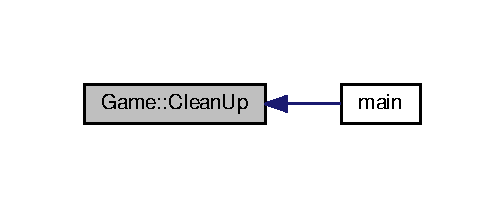
\includegraphics[width=242pt]{class_game_afe8f2a4980f240bbfba8c1f495ff5075_icgraph}
\end{center}
\end{figure}


\hypertarget{class_game_a6b7a69223477dbfae5f570763385a2f1}{}\index{Game@{Game}!Handle\+Events@{Handle\+Events}}
\index{Handle\+Events@{Handle\+Events}!Game@{Game}}
\subsubsection[{Handle\+Events}]{\setlength{\rightskip}{0pt plus 5cm}void Game\+::\+Handle\+Events (
\begin{DoxyParamCaption}
\item[{S\+D\+L\+\_\+\+Event}]{e, }
\item[{S\+D\+L\+\_\+\+Window $\ast$}]{\+\_\+window}
\end{DoxyParamCaption}
)}\label{class_game_a6b7a69223477dbfae5f570763385a2f1}


Here is the call graph for this function\+:\nopagebreak
\begin{figure}[H]
\begin{center}
\leavevmode
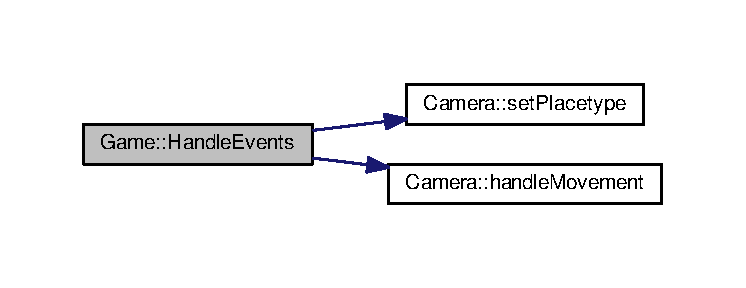
\includegraphics[width=350pt]{class_game_a6b7a69223477dbfae5f570763385a2f1_cgraph}
\end{center}
\end{figure}




Here is the caller graph for this function\+:\nopagebreak
\begin{figure}[H]
\begin{center}
\leavevmode
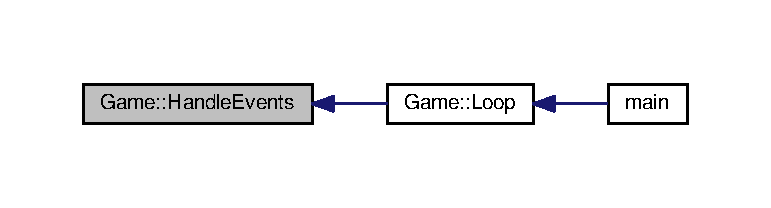
\includegraphics[width=350pt]{class_game_a6b7a69223477dbfae5f570763385a2f1_icgraph}
\end{center}
\end{figure}


\hypertarget{class_game_a555a9e4719fd49971765a2ab8b090b5c}{}\index{Game@{Game}!Init@{Init}}
\index{Init@{Init}!Game@{Game}}
\subsubsection[{Init}]{\setlength{\rightskip}{0pt plus 5cm}void Game\+::\+Init (
\begin{DoxyParamCaption}
{}
\end{DoxyParamCaption}
)}\label{class_game_a555a9e4719fd49971765a2ab8b090b5c}
Initialise subsytems and load data 

Here is the call graph for this function\+:\nopagebreak
\begin{figure}[H]
\begin{center}
\leavevmode
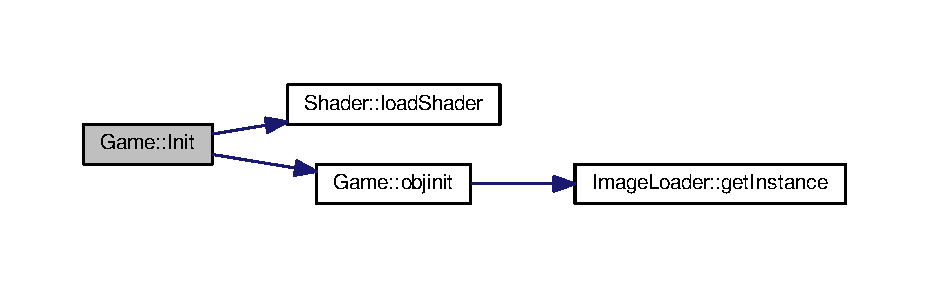
\includegraphics[width=350pt]{class_game_a555a9e4719fd49971765a2ab8b090b5c_cgraph}
\end{center}
\end{figure}




Here is the caller graph for this function\+:\nopagebreak
\begin{figure}[H]
\begin{center}
\leavevmode
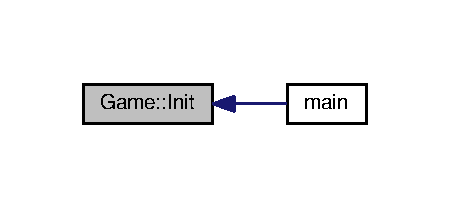
\includegraphics[width=216pt]{class_game_a555a9e4719fd49971765a2ab8b090b5c_icgraph}
\end{center}
\end{figure}


\hypertarget{class_game_a28d8a0a65bda89be42d9c46fc2e4f14b}{}\index{Game@{Game}!Loop@{Loop}}
\index{Loop@{Loop}!Game@{Game}}
\subsubsection[{Loop}]{\setlength{\rightskip}{0pt plus 5cm}void Game\+::\+Loop (
\begin{DoxyParamCaption}
{}
\end{DoxyParamCaption}
)}\label{class_game_a28d8a0a65bda89be42d9c46fc2e4f14b}
Main loop 

Here is the call graph for this function\+:\nopagebreak
\begin{figure}[H]
\begin{center}
\leavevmode
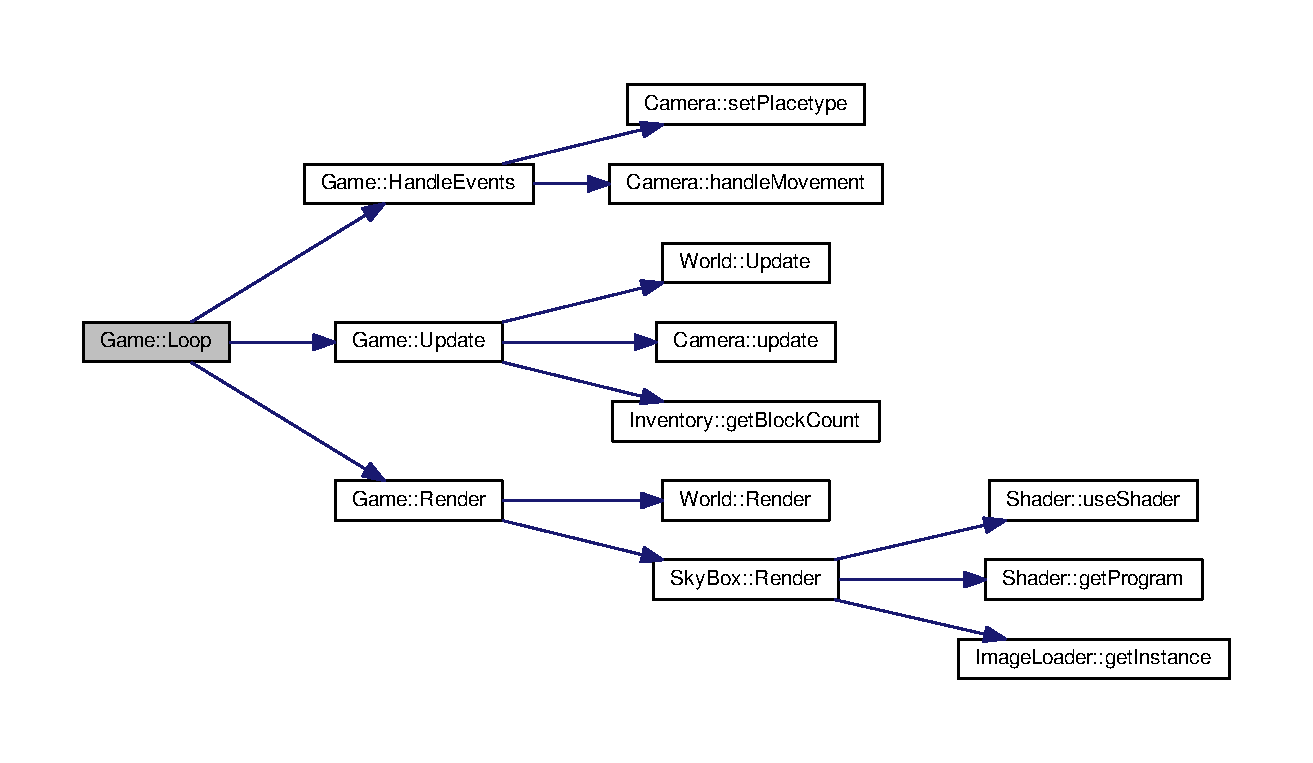
\includegraphics[width=350pt]{class_game_a28d8a0a65bda89be42d9c46fc2e4f14b_cgraph}
\end{center}
\end{figure}




Here is the caller graph for this function\+:\nopagebreak
\begin{figure}[H]
\begin{center}
\leavevmode
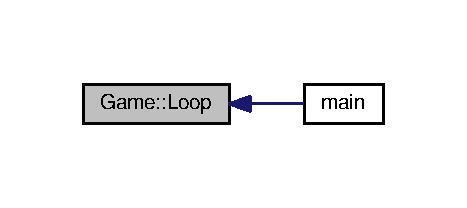
\includegraphics[width=224pt]{class_game_a28d8a0a65bda89be42d9c46fc2e4f14b_icgraph}
\end{center}
\end{figure}


\hypertarget{class_game_a7b9c3ffde53cdf3fa685d6e9b5ae43f3}{}\index{Game@{Game}!objinit@{objinit}}
\index{objinit@{objinit}!Game@{Game}}
\subsubsection[{objinit}]{\setlength{\rightskip}{0pt plus 5cm}void Game\+::objinit (
\begin{DoxyParamCaption}
{}
\end{DoxyParamCaption}
)}\label{class_game_a7b9c3ffde53cdf3fa685d6e9b5ae43f3}


Here is the call graph for this function\+:\nopagebreak
\begin{figure}[H]
\begin{center}
\leavevmode
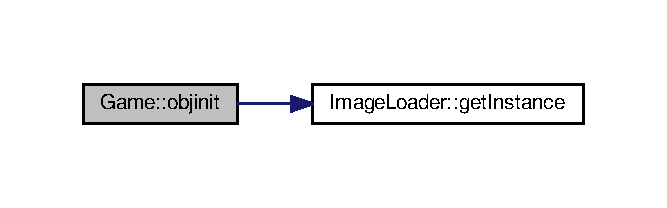
\includegraphics[width=320pt]{class_game_a7b9c3ffde53cdf3fa685d6e9b5ae43f3_cgraph}
\end{center}
\end{figure}




Here is the caller graph for this function\+:\nopagebreak
\begin{figure}[H]
\begin{center}
\leavevmode
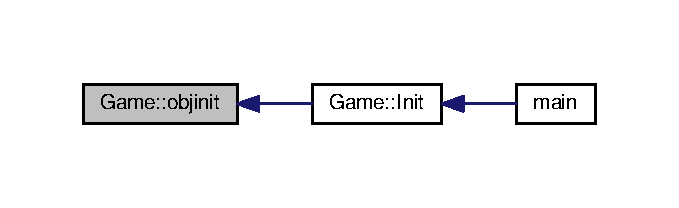
\includegraphics[width=326pt]{class_game_a7b9c3ffde53cdf3fa685d6e9b5ae43f3_icgraph}
\end{center}
\end{figure}


\hypertarget{class_game_a0897730fc9fed789f6c0f11d21a0c14a}{}\index{Game@{Game}!Render@{Render}}
\index{Render@{Render}!Game@{Game}}
\subsubsection[{Render}]{\setlength{\rightskip}{0pt plus 5cm}void Game\+::\+Render (
\begin{DoxyParamCaption}
{}
\end{DoxyParamCaption}
)}\label{class_game_a0897730fc9fed789f6c0f11d21a0c14a}


Here is the call graph for this function\+:\nopagebreak
\begin{figure}[H]
\begin{center}
\leavevmode
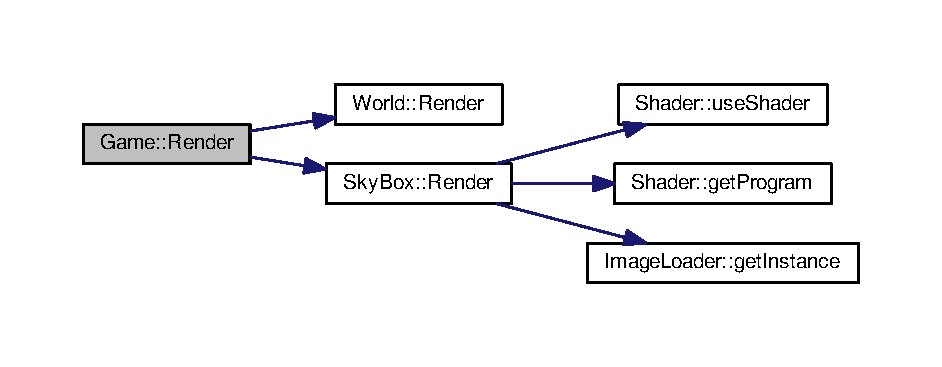
\includegraphics[width=350pt]{class_game_a0897730fc9fed789f6c0f11d21a0c14a_cgraph}
\end{center}
\end{figure}




Here is the caller graph for this function\+:\nopagebreak
\begin{figure}[H]
\begin{center}
\leavevmode
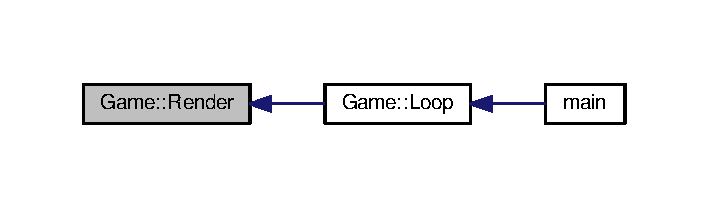
\includegraphics[width=340pt]{class_game_a0897730fc9fed789f6c0f11d21a0c14a_icgraph}
\end{center}
\end{figure}


\hypertarget{class_game_a1c5373c68261c54aff03e6abe40fee52}{}\index{Game@{Game}!Update@{Update}}
\index{Update@{Update}!Game@{Game}}
\subsubsection[{Update}]{\setlength{\rightskip}{0pt plus 5cm}void Game\+::\+Update (
\begin{DoxyParamCaption}
{}
\end{DoxyParamCaption}
)}\label{class_game_a1c5373c68261c54aff03e6abe40fee52}


Here is the call graph for this function\+:\nopagebreak
\begin{figure}[H]
\begin{center}
\leavevmode
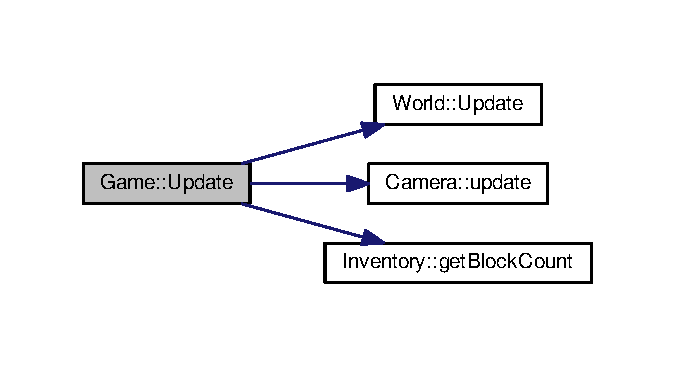
\includegraphics[width=324pt]{class_game_a1c5373c68261c54aff03e6abe40fee52_cgraph}
\end{center}
\end{figure}




Here is the caller graph for this function\+:\nopagebreak
\begin{figure}[H]
\begin{center}
\leavevmode
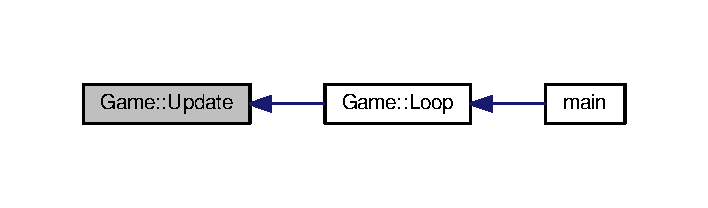
\includegraphics[width=340pt]{class_game_a1c5373c68261c54aff03e6abe40fee52_icgraph}
\end{center}
\end{figure}




\subsection{Member Data Documentation}
\hypertarget{class_game_ac93b435b5da2f81e01da94a2871c1394}{}\index{Game@{Game}!\+\_\+window@{\+\_\+window}}
\index{\+\_\+window@{\+\_\+window}!Game@{Game}}
\subsubsection[{\+\_\+window}]{\setlength{\rightskip}{0pt plus 5cm}S\+D\+L\+\_\+\+Window$\ast$ Game\+::\+\_\+window}\label{class_game_ac93b435b5da2f81e01da94a2871c1394}


The documentation for this class was generated from the following files\+:\begin{DoxyCompactItemize}
\item 
src/\hyperlink{_game_8h}{Game.\+h}\item 
src/\hyperlink{_game_8cpp}{Game.\+cpp}\end{DoxyCompactItemize}

\hypertarget{class_image_loader}{}\section{Image\+Loader Class Reference}
\label{class_image_loader}\index{Image\+Loader@{Image\+Loader}}


{\ttfamily \#include $<$Image\+Loader.\+h$>$}

\subsection*{Public Member Functions}
\begin{DoxyCompactItemize}
\item 
G\+Luint \hyperlink{class_image_loader_ab52b48518d13ff284d7d68bf7119d943}{Load\+Texture} (std\+::string filename)
\item 
\hyperlink{class_image_loader_a844109a0a6b4e4a9513fa6822f623dcc}{$\sim$\+Image\+Loader} ()
\item 
void \hyperlink{class_image_loader_adc8753fda50916c2e53d3e071502bb74}{Load\+Textures} ()
\item 
G\+Luint \hyperlink{class_image_loader_af71479e10a84606ab284ac1293436261}{Get\+Texture} (G\+Luint type)
\end{DoxyCompactItemize}
\subsection*{Static Public Member Functions}
\begin{DoxyCompactItemize}
\item 
static \hyperlink{class_image_loader}{Image\+Loader} $\ast$ \hyperlink{class_image_loader_adf162e4bf26be1abb849ce46f9634b69}{get\+Instance} ()
\end{DoxyCompactItemize}


\subsection{Detailed Description}
Singleton class for image handling 

\subsection{Constructor \& Destructor Documentation}
\hypertarget{class_image_loader_a844109a0a6b4e4a9513fa6822f623dcc}{}\index{Image\+Loader@{Image\+Loader}!````~Image\+Loader@{$\sim$\+Image\+Loader}}
\index{````~Image\+Loader@{$\sim$\+Image\+Loader}!Image\+Loader@{Image\+Loader}}
\subsubsection[{$\sim$\+Image\+Loader}]{\setlength{\rightskip}{0pt plus 5cm}Image\+Loader\+::$\sim$\+Image\+Loader (
\begin{DoxyParamCaption}
{}
\end{DoxyParamCaption}
)}\label{class_image_loader_a844109a0a6b4e4a9513fa6822f623dcc}


\subsection{Member Function Documentation}
\hypertarget{class_image_loader_adf162e4bf26be1abb849ce46f9634b69}{}\index{Image\+Loader@{Image\+Loader}!get\+Instance@{get\+Instance}}
\index{get\+Instance@{get\+Instance}!Image\+Loader@{Image\+Loader}}
\subsubsection[{get\+Instance}]{\setlength{\rightskip}{0pt plus 5cm}{\bf Image\+Loader} $\ast$ Image\+Loader\+::get\+Instance (
\begin{DoxyParamCaption}
{}
\end{DoxyParamCaption}
)\hspace{0.3cm}{\ttfamily [static]}}\label{class_image_loader_adf162e4bf26be1abb849ce46f9634b69}
Public access method If instance does not exist, crate it and return it, else just return it 

Here is the caller graph for this function\+:\nopagebreak
\begin{figure}[H]
\begin{center}
\leavevmode
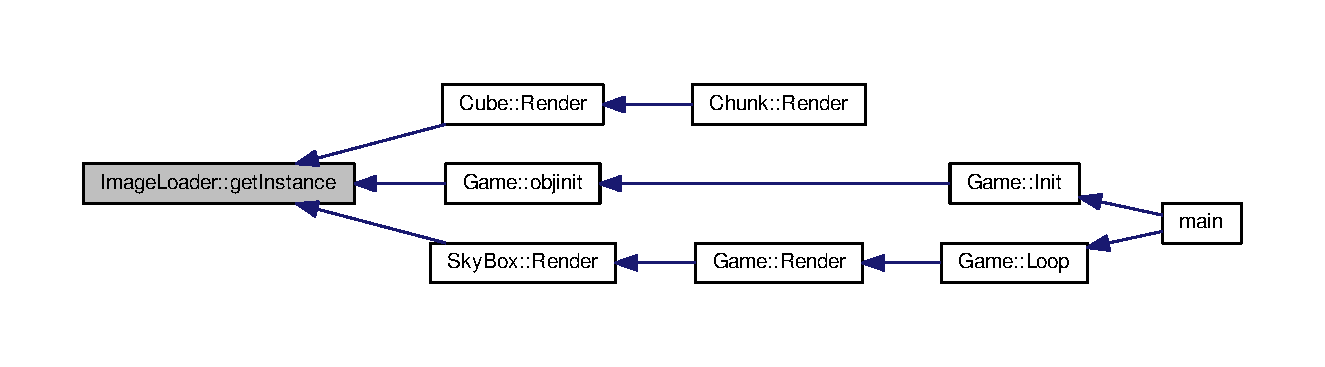
\includegraphics[width=350pt]{class_image_loader_adf162e4bf26be1abb849ce46f9634b69_icgraph}
\end{center}
\end{figure}


\hypertarget{class_image_loader_af71479e10a84606ab284ac1293436261}{}\index{Image\+Loader@{Image\+Loader}!Get\+Texture@{Get\+Texture}}
\index{Get\+Texture@{Get\+Texture}!Image\+Loader@{Image\+Loader}}
\subsubsection[{Get\+Texture}]{\setlength{\rightskip}{0pt plus 5cm}G\+Luint Image\+Loader\+::\+Get\+Texture (
\begin{DoxyParamCaption}
\item[{G\+Luint}]{type}
\end{DoxyParamCaption}
)}\label{class_image_loader_af71479e10a84606ab284ac1293436261}
Return texture type \hypertarget{class_image_loader_ab52b48518d13ff284d7d68bf7119d943}{}\index{Image\+Loader@{Image\+Loader}!Load\+Texture@{Load\+Texture}}
\index{Load\+Texture@{Load\+Texture}!Image\+Loader@{Image\+Loader}}
\subsubsection[{Load\+Texture}]{\setlength{\rightskip}{0pt plus 5cm}G\+Luint Image\+Loader\+::\+Load\+Texture (
\begin{DoxyParamCaption}
\item[{std\+::string}]{filename}
\end{DoxyParamCaption}
)}\label{class_image_loader_ab52b48518d13ff284d7d68bf7119d943}
Load image and generate opengl texture

Set texture parameters

Set texture filtering

Here is the caller graph for this function\+:\nopagebreak
\begin{figure}[H]
\begin{center}
\leavevmode
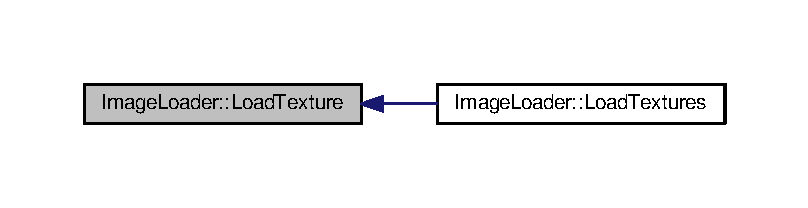
\includegraphics[width=350pt]{class_image_loader_ab52b48518d13ff284d7d68bf7119d943_icgraph}
\end{center}
\end{figure}


\hypertarget{class_image_loader_adc8753fda50916c2e53d3e071502bb74}{}\index{Image\+Loader@{Image\+Loader}!Load\+Textures@{Load\+Textures}}
\index{Load\+Textures@{Load\+Textures}!Image\+Loader@{Image\+Loader}}
\subsubsection[{Load\+Textures}]{\setlength{\rightskip}{0pt plus 5cm}void Image\+Loader\+::\+Load\+Textures (
\begin{DoxyParamCaption}
{}
\end{DoxyParamCaption}
)}\label{class_image_loader_adc8753fda50916c2e53d3e071502bb74}
Load all textures. 

Here is the call graph for this function\+:\nopagebreak
\begin{figure}[H]
\begin{center}
\leavevmode
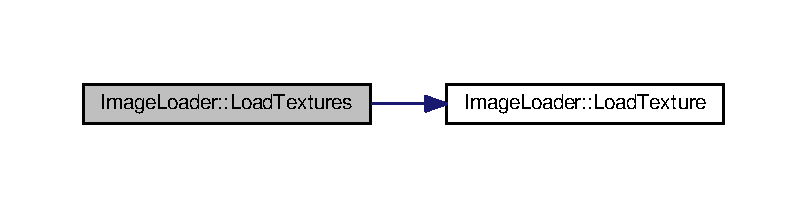
\includegraphics[width=350pt]{class_image_loader_adc8753fda50916c2e53d3e071502bb74_cgraph}
\end{center}
\end{figure}




The documentation for this class was generated from the following files\+:\begin{DoxyCompactItemize}
\item 
src/\hyperlink{_image_loader_8h}{Image\+Loader.\+h}\item 
src/\hyperlink{_image_loader_8cpp}{Image\+Loader.\+cpp}\end{DoxyCompactItemize}

\hypertarget{class_inventory}{}\section{Inventory Class Reference}
\label{class_inventory}\index{Inventory@{Inventory}}


{\ttfamily \#include $<$Inventory.\+h$>$}

\subsection*{Public Member Functions}
\begin{DoxyCompactItemize}
\item 
\hyperlink{class_inventory_a10485613fc8bfb32ee564d9b5110f8fb}{Inventory} ()
\item 
\hyperlink{class_inventory_a6c6dfcb6d977c74a7abf46809e892e3d}{$\sim$\+Inventory} ()
\item 
int \hyperlink{class_inventory_a463d58902824c007dc9a10ab54e9c671}{get\+Block\+Count} (G\+Luint type)
\item 
void \hyperlink{class_inventory_ad4526e79a12197311ff5a09cfe2f06b7}{inc\+Block\+Count} (G\+Luint type)
\item 
void \hyperlink{class_inventory_a985395e4e612f60ae9f6091af31dbfa4}{dec\+Block\+Count} (G\+Luint type)
\end{DoxyCompactItemize}


\subsection{Constructor \& Destructor Documentation}
\hypertarget{class_inventory_a10485613fc8bfb32ee564d9b5110f8fb}{}\index{Inventory@{Inventory}!Inventory@{Inventory}}
\index{Inventory@{Inventory}!Inventory@{Inventory}}
\subsubsection[{Inventory}]{\setlength{\rightskip}{0pt plus 5cm}Inventory\+::\+Inventory (
\begin{DoxyParamCaption}
{}
\end{DoxyParamCaption}
)}\label{class_inventory_a10485613fc8bfb32ee564d9b5110f8fb}
\hyperlink{class_inventory}{Inventory} constructor. Initialises block counts to 0. \hypertarget{class_inventory_a6c6dfcb6d977c74a7abf46809e892e3d}{}\index{Inventory@{Inventory}!````~Inventory@{$\sim$\+Inventory}}
\index{````~Inventory@{$\sim$\+Inventory}!Inventory@{Inventory}}
\subsubsection[{$\sim$\+Inventory}]{\setlength{\rightskip}{0pt plus 5cm}Inventory\+::$\sim$\+Inventory (
\begin{DoxyParamCaption}
{}
\end{DoxyParamCaption}
)}\label{class_inventory_a6c6dfcb6d977c74a7abf46809e892e3d}
Empty inventory destructor.

\begin{DoxyReturn}{Returns}
N\+U\+L\+L 
\end{DoxyReturn}


\subsection{Member Function Documentation}
\hypertarget{class_inventory_a985395e4e612f60ae9f6091af31dbfa4}{}\index{Inventory@{Inventory}!dec\+Block\+Count@{dec\+Block\+Count}}
\index{dec\+Block\+Count@{dec\+Block\+Count}!Inventory@{Inventory}}
\subsubsection[{dec\+Block\+Count}]{\setlength{\rightskip}{0pt plus 5cm}void Inventory\+::dec\+Block\+Count (
\begin{DoxyParamCaption}
\item[{G\+Luint}]{type}
\end{DoxyParamCaption}
)}\label{class_inventory_a985395e4e612f60ae9f6091af31dbfa4}
Method to decrement block count for a certain type.


\begin{DoxyParams}{Parameters}
{\em type} & -\/ Type of block to decrement count for.\\
\hline
\end{DoxyParams}
\begin{DoxyReturn}{Returns}
N\+U\+L\+L 
\end{DoxyReturn}


Here is the caller graph for this function\+:\nopagebreak
\begin{figure}[H]
\begin{center}
\leavevmode
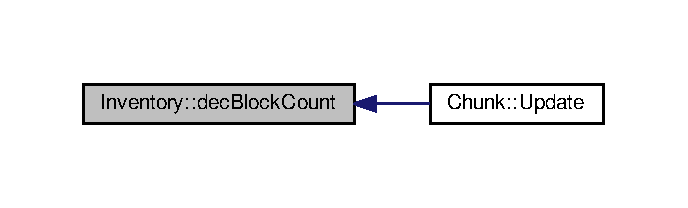
\includegraphics[width=330pt]{class_inventory_a985395e4e612f60ae9f6091af31dbfa4_icgraph}
\end{center}
\end{figure}


\hypertarget{class_inventory_a463d58902824c007dc9a10ab54e9c671}{}\index{Inventory@{Inventory}!get\+Block\+Count@{get\+Block\+Count}}
\index{get\+Block\+Count@{get\+Block\+Count}!Inventory@{Inventory}}
\subsubsection[{get\+Block\+Count}]{\setlength{\rightskip}{0pt plus 5cm}int Inventory\+::get\+Block\+Count (
\begin{DoxyParamCaption}
\item[{G\+Luint}]{type}
\end{DoxyParamCaption}
)}\label{class_inventory_a463d58902824c007dc9a10ab54e9c671}
\hyperlink{class_inventory}{Inventory} method to get block count of a certain type.


\begin{DoxyParams}{Parameters}
{\em type} & -\/ Type of block to get the count for.\\
\hline
\end{DoxyParams}
\begin{DoxyReturn}{Returns}
I\+N\+T -\/ number of blocks of passed in type. 
\end{DoxyReturn}


Here is the caller graph for this function\+:\nopagebreak
\begin{figure}[H]
\begin{center}
\leavevmode
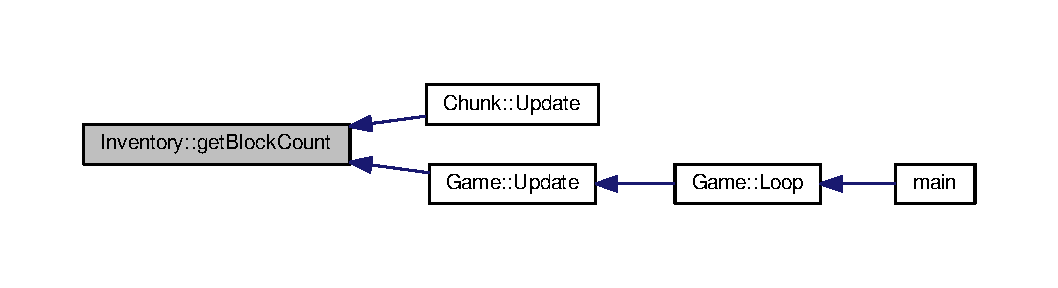
\includegraphics[width=350pt]{class_inventory_a463d58902824c007dc9a10ab54e9c671_icgraph}
\end{center}
\end{figure}


\hypertarget{class_inventory_ad4526e79a12197311ff5a09cfe2f06b7}{}\index{Inventory@{Inventory}!inc\+Block\+Count@{inc\+Block\+Count}}
\index{inc\+Block\+Count@{inc\+Block\+Count}!Inventory@{Inventory}}
\subsubsection[{inc\+Block\+Count}]{\setlength{\rightskip}{0pt plus 5cm}void Inventory\+::inc\+Block\+Count (
\begin{DoxyParamCaption}
\item[{G\+Luint}]{type}
\end{DoxyParamCaption}
)}\label{class_inventory_ad4526e79a12197311ff5a09cfe2f06b7}
Method to increment block count for a certain type.


\begin{DoxyParams}{Parameters}
{\em type} & -\/ Type of block to increment count for.\\
\hline
\end{DoxyParams}
\begin{DoxyReturn}{Returns}
N\+U\+L\+L 
\end{DoxyReturn}


Here is the caller graph for this function\+:\nopagebreak
\begin{figure}[H]
\begin{center}
\leavevmode
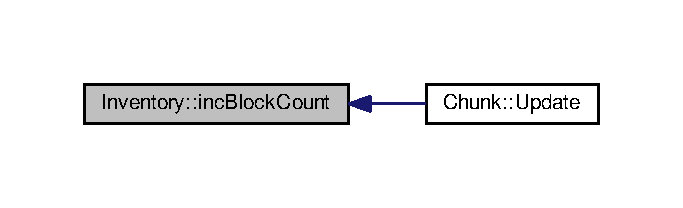
\includegraphics[width=328pt]{class_inventory_ad4526e79a12197311ff5a09cfe2f06b7_icgraph}
\end{center}
\end{figure}




The documentation for this class was generated from the following files\+:\begin{DoxyCompactItemize}
\item 
src/\hyperlink{_inventory_8h}{Inventory.\+h}\item 
src/\hyperlink{_inventory_8cpp}{Inventory.\+cpp}\end{DoxyCompactItemize}

\hypertarget{class_perlin}{}\section{Perlin Class Reference}
\label{class_perlin}\index{Perlin@{Perlin}}


{\ttfamily \#include $<$Perlin.\+h$>$}

\subsection*{Public Member Functions}
\begin{DoxyCompactItemize}
\item 
\hyperlink{class_perlin_af435cbd994560e90e5707fe841e3d2e1}{Perlin} ()
\item 
\hyperlink{class_perlin_a74c52ee250a2c10683b4ad3ac9ef2055}{$\sim$\+Perlin} ()
\item 
double \hyperlink{class_perlin_affd1073ebf50ec892e36805510df2792}{fade} (double t)
\item 
double \hyperlink{class_perlin_a2036993a6444693cf37dbde7dcdf023c}{noise} (double x, double y, double z)
\item 
double \hyperlink{class_perlin_a8143acc826a14ce25e864ecf68f62e73}{grad} (int hash, double x, double y, double z)
\item 
double \hyperlink{class_perlin_a2075b908242dbcd32eb45b31c5bf969f}{lerp} (double t, double a, double b)
\item 
double \hyperlink{class_perlin_a9279f30e21d3d19e0d4013e2cc797694}{octave} (double x, double y, double z, int octaves, double persistance)
\end{DoxyCompactItemize}


\subsection{Constructor \& Destructor Documentation}
\hypertarget{class_perlin_af435cbd994560e90e5707fe841e3d2e1}{}\index{Perlin@{Perlin}!Perlin@{Perlin}}
\index{Perlin@{Perlin}!Perlin@{Perlin}}
\subsubsection[{Perlin}]{\setlength{\rightskip}{0pt plus 5cm}Perlin\+::\+Perlin (
\begin{DoxyParamCaption}
{}
\end{DoxyParamCaption}
)}\label{class_perlin_af435cbd994560e90e5707fe841e3d2e1}
\hyperlink{class_perlin}{Perlin} constructor intialises the permutation vectors to a set random list. \hypertarget{class_perlin_a74c52ee250a2c10683b4ad3ac9ef2055}{}\index{Perlin@{Perlin}!````~Perlin@{$\sim$\+Perlin}}
\index{````~Perlin@{$\sim$\+Perlin}!Perlin@{Perlin}}
\subsubsection[{$\sim$\+Perlin}]{\setlength{\rightskip}{0pt plus 5cm}Perlin\+::$\sim$\+Perlin (
\begin{DoxyParamCaption}
{}
\end{DoxyParamCaption}
)}\label{class_perlin_a74c52ee250a2c10683b4ad3ac9ef2055}
\hyperlink{class_perlin}{Perlin} destructor. Does nothing. 

\subsection{Member Function Documentation}
\hypertarget{class_perlin_affd1073ebf50ec892e36805510df2792}{}\index{Perlin@{Perlin}!fade@{fade}}
\index{fade@{fade}!Perlin@{Perlin}}
\subsubsection[{fade}]{\setlength{\rightskip}{0pt plus 5cm}double Perlin\+::fade (
\begin{DoxyParamCaption}
\item[{double}]{t}
\end{DoxyParamCaption}
)}\label{class_perlin_affd1073ebf50ec892e36805510df2792}
\hyperlink{class_perlin}{Perlin} fade function. takes a parameter and mutates it then returns it.


\begin{DoxyParams}{Parameters}
{\em t} & -\/ value to fade\\
\hline
\end{DoxyParams}
\begin{DoxyReturn}{Returns}
D\+O\+U\+B\+L\+E -\/ faded value 
\end{DoxyReturn}


Here is the caller graph for this function\+:\nopagebreak
\begin{figure}[H]
\begin{center}
\leavevmode
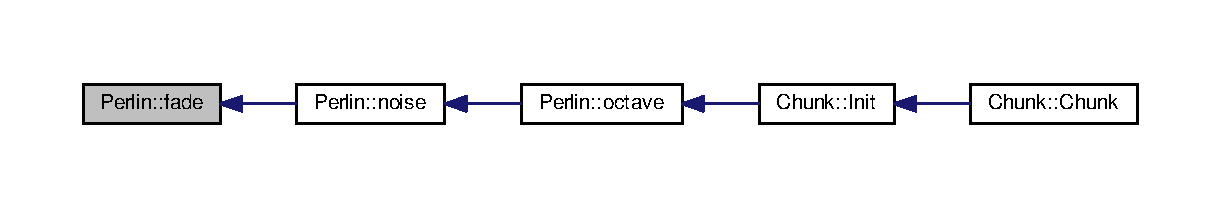
\includegraphics[width=350pt]{class_perlin_affd1073ebf50ec892e36805510df2792_icgraph}
\end{center}
\end{figure}


\hypertarget{class_perlin_a8143acc826a14ce25e864ecf68f62e73}{}\index{Perlin@{Perlin}!grad@{grad}}
\index{grad@{grad}!Perlin@{Perlin}}
\subsubsection[{grad}]{\setlength{\rightskip}{0pt plus 5cm}double Perlin\+::grad (
\begin{DoxyParamCaption}
\item[{int}]{hash, }
\item[{double}]{x, }
\item[{double}]{y, }
\item[{double}]{z}
\end{DoxyParamCaption}
)}\label{class_perlin_a8143acc826a14ce25e864ecf68f62e73}
Gradient function.


\begin{DoxyParams}{Parameters}
{\em hash} & -\/ The hash value used to return a gradient \\
\hline
{\em x} & -\/ x position we get a gradient for \\
\hline
{\em y} & -\/ y position we get a gradient for \\
\hline
{\em z} & -\/ z position we get a gradient for\\
\hline
\end{DoxyParams}
\begin{DoxyReturn}{Returns}
D\+O\+U\+B\+L\+E -\/ The calculated gradient 
\end{DoxyReturn}


Here is the caller graph for this function\+:\nopagebreak
\begin{figure}[H]
\begin{center}
\leavevmode
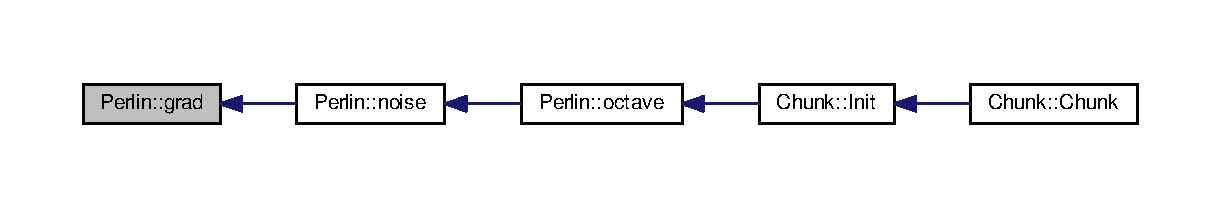
\includegraphics[width=350pt]{class_perlin_a8143acc826a14ce25e864ecf68f62e73_icgraph}
\end{center}
\end{figure}


\hypertarget{class_perlin_a2075b908242dbcd32eb45b31c5bf969f}{}\index{Perlin@{Perlin}!lerp@{lerp}}
\index{lerp@{lerp}!Perlin@{Perlin}}
\subsubsection[{lerp}]{\setlength{\rightskip}{0pt plus 5cm}double Perlin\+::lerp (
\begin{DoxyParamCaption}
\item[{double}]{t, }
\item[{double}]{a, }
\item[{double}]{b}
\end{DoxyParamCaption}
)}\label{class_perlin_a2075b908242dbcd32eb45b31c5bf969f}
A lerp function. i.\+e. linear interpolation between two points.


\begin{DoxyParams}{Parameters}
{\em t} & -\/ constant value \\
\hline
{\em a} & -\/ value to lerp from \\
\hline
{\em b} & -\/ value to lerp too\\
\hline
\end{DoxyParams}
\begin{DoxyReturn}{Returns}
D\+O\+U\+B\+L\+E -\/ the resulting lerp. 
\end{DoxyReturn}


Here is the caller graph for this function\+:\nopagebreak
\begin{figure}[H]
\begin{center}
\leavevmode
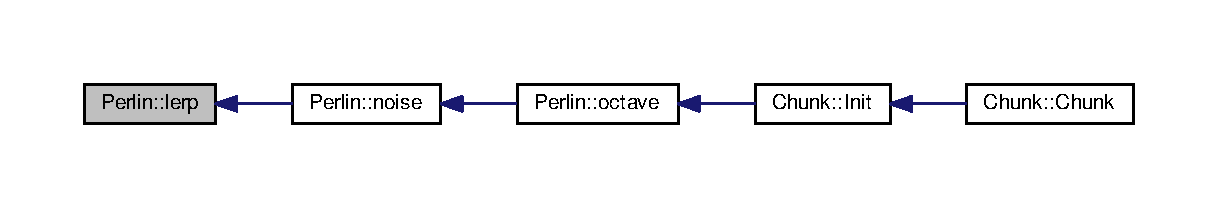
\includegraphics[width=350pt]{class_perlin_a2075b908242dbcd32eb45b31c5bf969f_icgraph}
\end{center}
\end{figure}


\hypertarget{class_perlin_a2036993a6444693cf37dbde7dcdf023c}{}\index{Perlin@{Perlin}!noise@{noise}}
\index{noise@{noise}!Perlin@{Perlin}}
\subsubsection[{noise}]{\setlength{\rightskip}{0pt plus 5cm}double Perlin\+::noise (
\begin{DoxyParamCaption}
\item[{double}]{x, }
\item[{double}]{y, }
\item[{double}]{z}
\end{DoxyParamCaption}
)}\label{class_perlin_a2036993a6444693cf37dbde7dcdf023c}
The actual noise function. Returns a value between -\/1 and 1.


\begin{DoxyParams}{Parameters}
{\em x} & -\/ x value of the position the noise is wanted for. \\
\hline
{\em y} & -\/ y value of the position the noise is wanted for. \\
\hline
{\em z} & -\/ z value of the position the noise is wanted for. This value can be a set value to get 2\+D noise.\\
\hline
\end{DoxyParams}
\begin{DoxyReturn}{Returns}
D\+O\+U\+B\+L\+E -\/ Noise for a certain position for (X, Y, Z) 
\end{DoxyReturn}


Here is the call graph for this function\+:\nopagebreak
\begin{figure}[H]
\begin{center}
\leavevmode
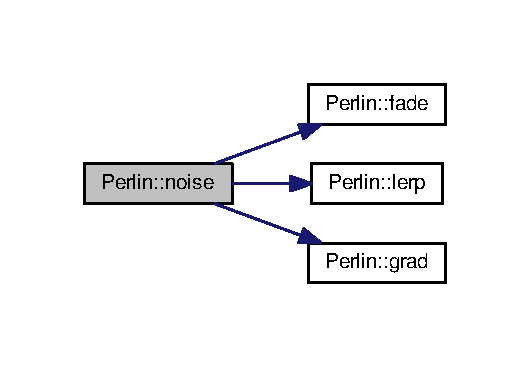
\includegraphics[width=254pt]{class_perlin_a2036993a6444693cf37dbde7dcdf023c_cgraph}
\end{center}
\end{figure}




Here is the caller graph for this function\+:\nopagebreak
\begin{figure}[H]
\begin{center}
\leavevmode
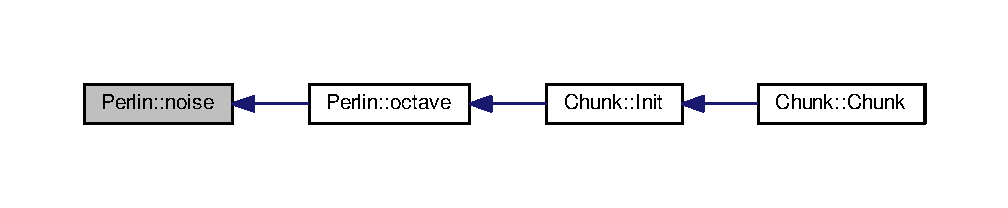
\includegraphics[width=350pt]{class_perlin_a2036993a6444693cf37dbde7dcdf023c_icgraph}
\end{center}
\end{figure}


\hypertarget{class_perlin_a9279f30e21d3d19e0d4013e2cc797694}{}\index{Perlin@{Perlin}!octave@{octave}}
\index{octave@{octave}!Perlin@{Perlin}}
\subsubsection[{octave}]{\setlength{\rightskip}{0pt plus 5cm}double Perlin\+::octave (
\begin{DoxyParamCaption}
\item[{double}]{x, }
\item[{double}]{y, }
\item[{double}]{z, }
\item[{int}]{octaves, }
\item[{double}]{persistance}
\end{DoxyParamCaption}
)}\label{class_perlin_a9279f30e21d3d19e0d4013e2cc797694}
A function to produce noise for multiple octaves.


\begin{DoxyParams}{Parameters}
{\em x} & -\/ x position of noise \\
\hline
{\em y} & -\/ y position of noise \\
\hline
{\em z} & -\/ z position of noise -\/ can be constant value for 2\+D noise \\
\hline
{\em octaves} & -\/ number of octaves wanted \\
\hline
{\em persistence} & -\/ how persistent should this function be? usually between 0 and 1.\+0.\\
\hline
\end{DoxyParams}
\begin{DoxyReturn}{Returns}
D\+O\+U\+B\+L\+E octave noise for (x, y, z) position 
\end{DoxyReturn}


Here is the call graph for this function\+:\nopagebreak
\begin{figure}[H]
\begin{center}
\leavevmode
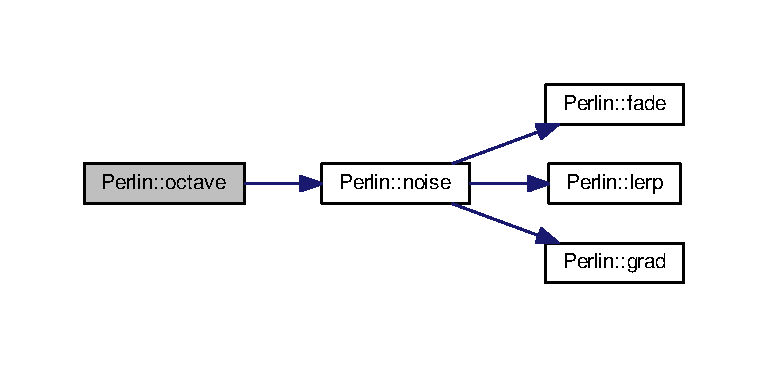
\includegraphics[width=350pt]{class_perlin_a9279f30e21d3d19e0d4013e2cc797694_cgraph}
\end{center}
\end{figure}




Here is the caller graph for this function\+:\nopagebreak
\begin{figure}[H]
\begin{center}
\leavevmode
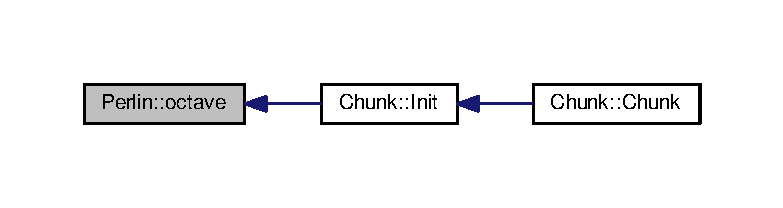
\includegraphics[width=350pt]{class_perlin_a9279f30e21d3d19e0d4013e2cc797694_icgraph}
\end{center}
\end{figure}




The documentation for this class was generated from the following files\+:\begin{DoxyCompactItemize}
\item 
src/\hyperlink{_perlin_8h}{Perlin.\+h}\item 
src/\hyperlink{_perlin_8cpp}{Perlin.\+cpp}\end{DoxyCompactItemize}

\hypertarget{class_ray_cast}{}\section{Ray\+Cast Class Reference}
\label{class_ray_cast}\index{Ray\+Cast@{Ray\+Cast}}


{\ttfamily \#include $<$Ray\+Cast.\+h$>$}

\subsection*{Public Member Functions}
\begin{DoxyCompactItemize}
\item 
void \hyperlink{class_ray_cast_a87834fb8de45433e8525936d08885613}{get\+Ray} (int x, int y)
\end{DoxyCompactItemize}


\subsection{Member Function Documentation}
\hypertarget{class_ray_cast_a87834fb8de45433e8525936d08885613}{}\index{Ray\+Cast@{Ray\+Cast}!get\+Ray@{get\+Ray}}
\index{get\+Ray@{get\+Ray}!Ray\+Cast@{Ray\+Cast}}
\subsubsection[{get\+Ray}]{\setlength{\rightskip}{0pt plus 5cm}void Ray\+Cast\+::get\+Ray (
\begin{DoxyParamCaption}
\item[{int}]{x, }
\item[{int}]{y}
\end{DoxyParamCaption}
)}\label{class_ray_cast_a87834fb8de45433e8525936d08885613}


The documentation for this class was generated from the following files\+:\begin{DoxyCompactItemize}
\item 
src/\hyperlink{_ray_cast_8h}{Ray\+Cast.\+h}\item 
src/\hyperlink{_ray_cast_8cpp}{Ray\+Cast.\+cpp}\end{DoxyCompactItemize}

\hypertarget{class_shader}{}\section{Shader Class Reference}
\label{class_shader}\index{Shader@{Shader}}


{\ttfamily \#include $<$Shader.\+h$>$}

\subsection*{Public Member Functions}
\begin{DoxyCompactItemize}
\item 
\hyperlink{class_shader_a0d654ebaca4e0555197c0724c6d30610}{Shader} ()
\item 
\hyperlink{class_shader_aff01df87e8a102f270b5b135a295e59d}{$\sim$\+Shader} ()
\item 
void \hyperlink{class_shader_a19a6341e1d67136647556d9cff3c2242}{load\+Shader} (std\+::string v\+Filename, std\+::string f\+Filename)
\item 
void \hyperlink{class_shader_a6212f8a189b932362d1f6cffb31b6633}{use\+Shader} ()
\item 
G\+Luint \hyperlink{class_shader_ab3b6ebf2670424320d518f417a676fc2}{get\+Program} ()
\end{DoxyCompactItemize}


\subsection{Detailed Description}
\hyperlink{class_shader}{Shader} class 

\subsection{Constructor \& Destructor Documentation}
\hypertarget{class_shader_a0d654ebaca4e0555197c0724c6d30610}{}\index{Shader@{Shader}!Shader@{Shader}}
\index{Shader@{Shader}!Shader@{Shader}}
\subsubsection[{Shader}]{\setlength{\rightskip}{0pt plus 5cm}Shader\+::\+Shader (
\begin{DoxyParamCaption}
{}
\end{DoxyParamCaption}
)}\label{class_shader_a0d654ebaca4e0555197c0724c6d30610}
\hypertarget{class_shader_aff01df87e8a102f270b5b135a295e59d}{}\index{Shader@{Shader}!````~Shader@{$\sim$\+Shader}}
\index{````~Shader@{$\sim$\+Shader}!Shader@{Shader}}
\subsubsection[{$\sim$\+Shader}]{\setlength{\rightskip}{0pt plus 5cm}Shader\+::$\sim$\+Shader (
\begin{DoxyParamCaption}
{}
\end{DoxyParamCaption}
)}\label{class_shader_aff01df87e8a102f270b5b135a295e59d}


\subsection{Member Function Documentation}
\hypertarget{class_shader_ab3b6ebf2670424320d518f417a676fc2}{}\index{Shader@{Shader}!get\+Program@{get\+Program}}
\index{get\+Program@{get\+Program}!Shader@{Shader}}
\subsubsection[{get\+Program}]{\setlength{\rightskip}{0pt plus 5cm}G\+Luint Shader\+::get\+Program (
\begin{DoxyParamCaption}
{}
\end{DoxyParamCaption}
)}\label{class_shader_ab3b6ebf2670424320d518f417a676fc2}


Here is the caller graph for this function\+:\nopagebreak
\begin{figure}[H]
\begin{center}
\leavevmode
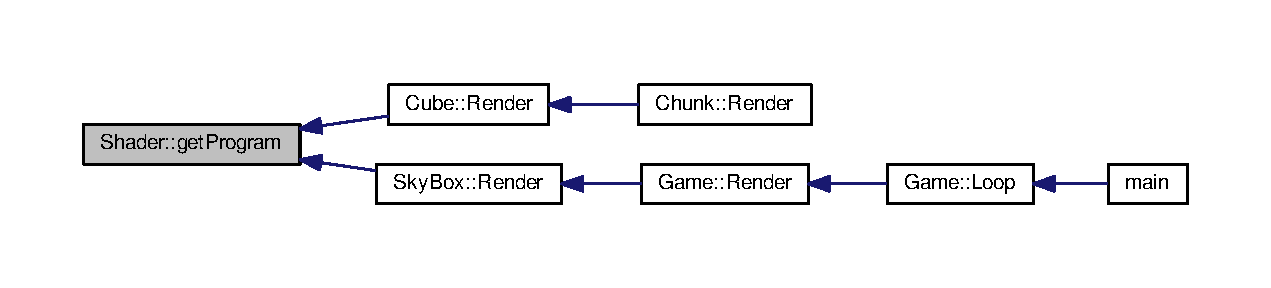
\includegraphics[width=350pt]{class_shader_ab3b6ebf2670424320d518f417a676fc2_icgraph}
\end{center}
\end{figure}


\hypertarget{class_shader_a19a6341e1d67136647556d9cff3c2242}{}\index{Shader@{Shader}!load\+Shader@{load\+Shader}}
\index{load\+Shader@{load\+Shader}!Shader@{Shader}}
\subsubsection[{load\+Shader}]{\setlength{\rightskip}{0pt plus 5cm}void Shader\+::load\+Shader (
\begin{DoxyParamCaption}
\item[{std\+::string}]{v\+Filename, }
\item[{std\+::string}]{f\+Filename}
\end{DoxyParamCaption}
)}\label{class_shader_a19a6341e1d67136647556d9cff3c2242}


Here is the caller graph for this function\+:\nopagebreak
\begin{figure}[H]
\begin{center}
\leavevmode
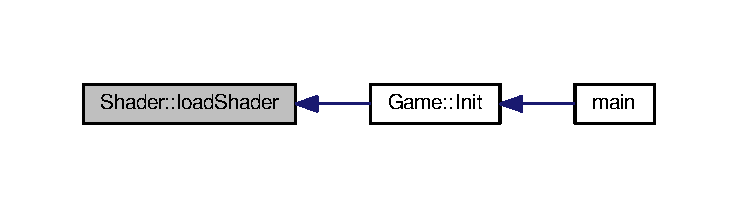
\includegraphics[width=350pt]{class_shader_a19a6341e1d67136647556d9cff3c2242_icgraph}
\end{center}
\end{figure}


\hypertarget{class_shader_a6212f8a189b932362d1f6cffb31b6633}{}\index{Shader@{Shader}!use\+Shader@{use\+Shader}}
\index{use\+Shader@{use\+Shader}!Shader@{Shader}}
\subsubsection[{use\+Shader}]{\setlength{\rightskip}{0pt plus 5cm}void Shader\+::use\+Shader (
\begin{DoxyParamCaption}
{}
\end{DoxyParamCaption}
)}\label{class_shader_a6212f8a189b932362d1f6cffb31b6633}


Here is the caller graph for this function\+:\nopagebreak
\begin{figure}[H]
\begin{center}
\leavevmode
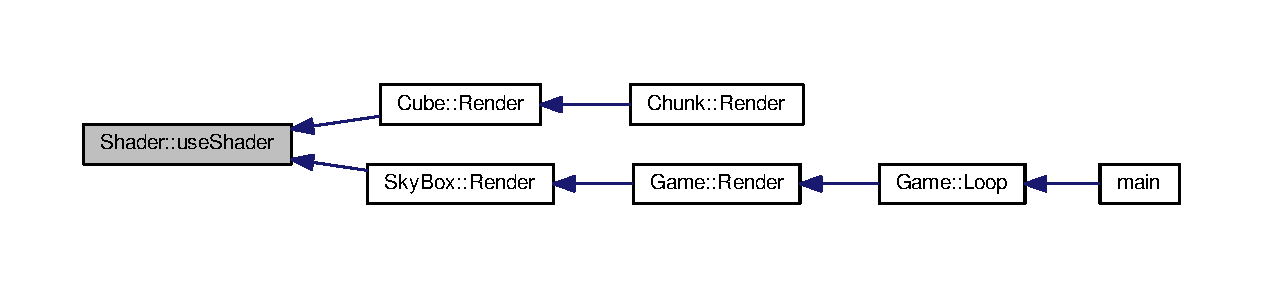
\includegraphics[width=350pt]{class_shader_a6212f8a189b932362d1f6cffb31b6633_icgraph}
\end{center}
\end{figure}




The documentation for this class was generated from the following files\+:\begin{DoxyCompactItemize}
\item 
src/\hyperlink{_shader_8h}{Shader.\+h}\item 
src/\hyperlink{_shader_8cpp}{Shader.\+cpp}\end{DoxyCompactItemize}

\hypertarget{class_sky_box}{}\section{Sky\+Box Class Reference}
\label{class_sky_box}\index{Sky\+Box@{Sky\+Box}}


{\ttfamily \#include $<$Sky\+Box.\+h$>$}

\subsection*{Public Member Functions}
\begin{DoxyCompactItemize}
\item 
\hyperlink{class_sky_box_a548db645757da94296cb80402206dd3b}{Sky\+Box} ()
\item 
\hyperlink{class_sky_box_aef6a9b7d384358fd2095d1e171d8a997}{$\sim$\+Sky\+Box} ()
\item 
void \hyperlink{class_sky_box_a95c75c3c40102bf9a1a4ca9980c609d5}{load\+Sky\+Box} ()
\item 
void \hyperlink{class_sky_box_af5f74045e6fb7761699a5b60aa4c38ef}{Render} (\hyperlink{class_shader}{Shader} shader, \hyperlink{class_camera}{Camera} $\ast$camera)
\item 
void \hyperlink{class_sky_box_a17d52c20c04d83aa3befaa4d40a37dd7}{set\+Position} (glm\+::vec3 pos)
\item 
glm\+::vec3 \hyperlink{class_sky_box_aa4905c9e9f9ffd8c3f46397d9a324644}{get\+Position} ()
\item 
G\+Luint \hyperlink{class_sky_box_a7cba71a3279e0988707cc72e170d50b8}{get\+Texture} ()
\end{DoxyCompactItemize}


\subsection{Constructor \& Destructor Documentation}
\hypertarget{class_sky_box_a548db645757da94296cb80402206dd3b}{}\index{Sky\+Box@{Sky\+Box}!Sky\+Box@{Sky\+Box}}
\index{Sky\+Box@{Sky\+Box}!Sky\+Box@{Sky\+Box}}
\subsubsection[{Sky\+Box}]{\setlength{\rightskip}{0pt plus 5cm}Sky\+Box\+::\+Sky\+Box (
\begin{DoxyParamCaption}
{}
\end{DoxyParamCaption}
)}\label{class_sky_box_a548db645757da94296cb80402206dd3b}
Skybox constructor initialises values.

then loads skybox. 

Here is the call graph for this function\+:\nopagebreak
\begin{figure}[H]
\begin{center}
\leavevmode
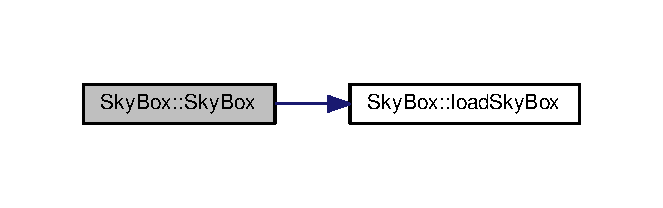
\includegraphics[width=318pt]{class_sky_box_a548db645757da94296cb80402206dd3b_cgraph}
\end{center}
\end{figure}


\hypertarget{class_sky_box_aef6a9b7d384358fd2095d1e171d8a997}{}\index{Sky\+Box@{Sky\+Box}!````~Sky\+Box@{$\sim$\+Sky\+Box}}
\index{````~Sky\+Box@{$\sim$\+Sky\+Box}!Sky\+Box@{Sky\+Box}}
\subsubsection[{$\sim$\+Sky\+Box}]{\setlength{\rightskip}{0pt plus 5cm}Sky\+Box\+::$\sim$\+Sky\+Box (
\begin{DoxyParamCaption}
{}
\end{DoxyParamCaption}
)}\label{class_sky_box_aef6a9b7d384358fd2095d1e171d8a997}
Skybox destructor. 

\subsection{Member Function Documentation}
\hypertarget{class_sky_box_aa4905c9e9f9ffd8c3f46397d9a324644}{}\index{Sky\+Box@{Sky\+Box}!get\+Position@{get\+Position}}
\index{get\+Position@{get\+Position}!Sky\+Box@{Sky\+Box}}
\subsubsection[{get\+Position}]{\setlength{\rightskip}{0pt plus 5cm}glm\+::vec3 Sky\+Box\+::get\+Position (
\begin{DoxyParamCaption}
{}
\end{DoxyParamCaption}
)\hspace{0.3cm}{\ttfamily [inline]}}\label{class_sky_box_aa4905c9e9f9ffd8c3f46397d9a324644}
\hypertarget{class_sky_box_a7cba71a3279e0988707cc72e170d50b8}{}\index{Sky\+Box@{Sky\+Box}!get\+Texture@{get\+Texture}}
\index{get\+Texture@{get\+Texture}!Sky\+Box@{Sky\+Box}}
\subsubsection[{get\+Texture}]{\setlength{\rightskip}{0pt plus 5cm}G\+Luint Sky\+Box\+::get\+Texture (
\begin{DoxyParamCaption}
{}
\end{DoxyParamCaption}
)\hspace{0.3cm}{\ttfamily [inline]}}\label{class_sky_box_a7cba71a3279e0988707cc72e170d50b8}
\hypertarget{class_sky_box_a95c75c3c40102bf9a1a4ca9980c609d5}{}\index{Sky\+Box@{Sky\+Box}!load\+Sky\+Box@{load\+Sky\+Box}}
\index{load\+Sky\+Box@{load\+Sky\+Box}!Sky\+Box@{Sky\+Box}}
\subsubsection[{load\+Sky\+Box}]{\setlength{\rightskip}{0pt plus 5cm}void Sky\+Box\+::load\+Sky\+Box (
\begin{DoxyParamCaption}
{}
\end{DoxyParamCaption}
)}\label{class_sky_box_a95c75c3c40102bf9a1a4ca9980c609d5}
Loads skybox into the V\+A\+O and V\+B\+O. which gets passed to the shader program later.

\begin{DoxyReturn}{Returns}
N\+U\+L\+L 
\end{DoxyReturn}


Here is the caller graph for this function\+:\nopagebreak
\begin{figure}[H]
\begin{center}
\leavevmode
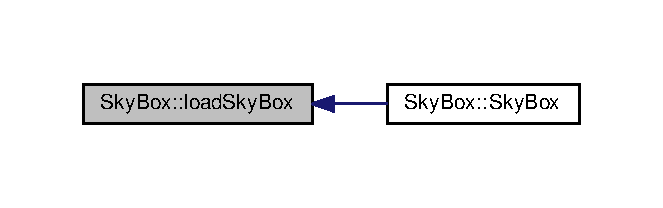
\includegraphics[width=318pt]{class_sky_box_a95c75c3c40102bf9a1a4ca9980c609d5_icgraph}
\end{center}
\end{figure}


\hypertarget{class_sky_box_af5f74045e6fb7761699a5b60aa4c38ef}{}\index{Sky\+Box@{Sky\+Box}!Render@{Render}}
\index{Render@{Render}!Sky\+Box@{Sky\+Box}}
\subsubsection[{Render}]{\setlength{\rightskip}{0pt plus 5cm}void Sky\+Box\+::\+Render (
\begin{DoxyParamCaption}
\item[{{\bf Shader}}]{shader, }
\item[{{\bf Camera} $\ast$}]{camera}
\end{DoxyParamCaption}
)}\label{class_sky_box_af5f74045e6fb7761699a5b60aa4c38ef}
Skybox render function. U\+Ses shader program and V\+B\+O/\+V\+A\+O to render skybox to screen.


\begin{DoxyParams}{Parameters}
{\em shader} & -\/ the shader program that will be used to render the skybox \\
\hline
{\em camera} & -\/ camera that will see the skybox when rendered.\\
\hline
\end{DoxyParams}
\begin{DoxyReturn}{Returns}
N\+U\+L\+L 
\end{DoxyReturn}


Here is the call graph for this function\+:\nopagebreak
\begin{figure}[H]
\begin{center}
\leavevmode
\includegraphics[width=336pt]{class_sky_box_af5f74045e6fb7761699a5b60aa4c38ef_cgraph}
\end{center}
\end{figure}




Here is the caller graph for this function\+:\nopagebreak
\begin{figure}[H]
\begin{center}
\leavevmode
\includegraphics[width=350pt]{class_sky_box_af5f74045e6fb7761699a5b60aa4c38ef_icgraph}
\end{center}
\end{figure}


\hypertarget{class_sky_box_a17d52c20c04d83aa3befaa4d40a37dd7}{}\index{Sky\+Box@{Sky\+Box}!set\+Position@{set\+Position}}
\index{set\+Position@{set\+Position}!Sky\+Box@{Sky\+Box}}
\subsubsection[{set\+Position}]{\setlength{\rightskip}{0pt plus 5cm}void Sky\+Box\+::set\+Position (
\begin{DoxyParamCaption}
\item[{glm\+::vec3}]{pos}
\end{DoxyParamCaption}
)\hspace{0.3cm}{\ttfamily [inline]}}\label{class_sky_box_a17d52c20c04d83aa3befaa4d40a37dd7}


The documentation for this class was generated from the following files\+:\begin{DoxyCompactItemize}
\item 
src/\hyperlink{_sky_box_8h}{Sky\+Box.\+h}\item 
src/\hyperlink{_sky_box_8cpp}{Sky\+Box.\+cpp}\end{DoxyCompactItemize}

\hypertarget{class_world}{}\section{World Class Reference}
\label{class_world}\index{World@{World}}


{\ttfamily \#include $<$World.\+h$>$}

\subsection*{Public Member Functions}
\begin{DoxyCompactItemize}
\item 
\hyperlink{class_world_afa39d4e6f714a7a3691ac0c656f5e8a8}{World} ()
\item 
\hyperlink{class_world_a8c73fba541a5817fff65147ba47cd827}{$\sim$\+World} ()
\item 
void \hyperlink{class_world_a48ae860aaeca4178c206900fa6a7871b}{Update} (\hyperlink{class_camera}{Camera} $\ast$camera)
\item 
void \hyperlink{class_world_adf195d52a1580150e1ca155f32a6b51a}{Render} (\hyperlink{class_shader}{Shader} shader, \hyperlink{class_camera}{Camera} $\ast$camera)
\end{DoxyCompactItemize}


\subsection{Constructor \& Destructor Documentation}
\hypertarget{class_world_afa39d4e6f714a7a3691ac0c656f5e8a8}{}\index{World@{World}!World@{World}}
\index{World@{World}!World@{World}}
\subsubsection[{World}]{\setlength{\rightskip}{0pt plus 5cm}World\+::\+World (
\begin{DoxyParamCaption}
{}
\end{DoxyParamCaption}
)}\label{class_world_afa39d4e6f714a7a3691ac0c656f5e8a8}
On creation \hyperlink{class_world}{World} needs to create 9 chunks i.\+e. chunk (0,0) and all 8 surrounding chunks. E.\+G. -\/ If X is (0,0) +++ +\+X+ +++ So chunks created are\+: ( 1,-\/1), ( 1,0), ( 1,1) ( 0,-\/1), ( 0,0), ( 0,1) (-\/1,-\/1), (-\/1,0), (-\/1,1) \hypertarget{class_world_a8c73fba541a5817fff65147ba47cd827}{}\index{World@{World}!````~World@{$\sim$\+World}}
\index{````~World@{$\sim$\+World}!World@{World}}
\subsubsection[{$\sim$\+World}]{\setlength{\rightskip}{0pt plus 5cm}World\+::$\sim$\+World (
\begin{DoxyParamCaption}
{}
\end{DoxyParamCaption}
)}\label{class_world_a8c73fba541a5817fff65147ba47cd827}
\hyperlink{class_world}{World} destructor. 

\subsection{Member Function Documentation}
\hypertarget{class_world_adf195d52a1580150e1ca155f32a6b51a}{}\index{World@{World}!Render@{Render}}
\index{Render@{Render}!World@{World}}
\subsubsection[{Render}]{\setlength{\rightskip}{0pt plus 5cm}void World\+::\+Render (
\begin{DoxyParamCaption}
\item[{{\bf Shader}}]{shader, }
\item[{{\bf Camera} $\ast$}]{camera}
\end{DoxyParamCaption}
)}\label{class_world_adf195d52a1580150e1ca155f32a6b51a}
Render should call each of the 9 loaded chunks own render method.


\begin{DoxyParams}{Parameters}
{\em shader} & -\/ the shader used to render the chunks \\
\hline
{\em camera} & -\/ teh camera that sees the chunks\\
\hline
\end{DoxyParams}
\begin{DoxyReturn}{Returns}
N\+U\+L\+L 
\end{DoxyReturn}


Here is the caller graph for this function\+:\nopagebreak
\begin{figure}[H]
\begin{center}
\leavevmode
\includegraphics[width=350pt]{class_world_adf195d52a1580150e1ca155f32a6b51a_icgraph}
\end{center}
\end{figure}


\hypertarget{class_world_a48ae860aaeca4178c206900fa6a7871b}{}\index{World@{World}!Update@{Update}}
\index{Update@{Update}!World@{World}}
\subsubsection[{Update}]{\setlength{\rightskip}{0pt plus 5cm}void World\+::\+Update (
\begin{DoxyParamCaption}
\item[{{\bf Camera} $\ast$}]{camera}
\end{DoxyParamCaption}
)}\label{class_world_a48ae860aaeca4178c206900fa6a7871b}
Update will find the chunk the player is in and check that all 8 surrounding chunks are loaded. If they arne\textquotesingle{}t it will load them. If they are it will do nothing.


\begin{DoxyParams}{Parameters}
{\em camera} & -\/ camera that collides with chunks\\
\hline
\end{DoxyParams}
\begin{DoxyReturn}{Returns}
N\+U\+L\+L 
\end{DoxyReturn}


Here is the caller graph for this function\+:\nopagebreak
\begin{figure}[H]
\begin{center}
\leavevmode
\includegraphics[width=350pt]{class_world_a48ae860aaeca4178c206900fa6a7871b_icgraph}
\end{center}
\end{figure}




The documentation for this class was generated from the following files\+:\begin{DoxyCompactItemize}
\item 
src/\hyperlink{_world_8h}{World.\+h}\item 
src/\hyperlink{_world_8cpp}{World.\+cpp}\end{DoxyCompactItemize}

\chapter{File Documentation}
\hypertarget{_camera_8cpp}{}\section{src/\+Camera.cpp File Reference}
\label{_camera_8cpp}\index{src/\+Camera.\+cpp@{src/\+Camera.\+cpp}}
{\ttfamily \#include \char`\"{}Camera.\+h\char`\"{}}\\*
Include dependency graph for Camera.\+cpp\+:\nopagebreak
\begin{figure}[H]
\begin{center}
\leavevmode
\includegraphics[width=350pt]{_camera_8cpp__incl}
\end{center}
\end{figure}

\hypertarget{_camera_8h}{}\section{src/\+Camera.h File Reference}
\label{_camera_8h}\index{src/\+Camera.\+h@{src/\+Camera.\+h}}
{\ttfamily \#include \char`\"{}S\+D\+L2/\+S\+D\+L.\+h\char`\"{}}\\*
{\ttfamily \#include \char`\"{}G\+L/glew.\+h\char`\"{}}\\*
{\ttfamily \#include \char`\"{}G\+L/glu.\+h\char`\"{}}\\*
{\ttfamily \#include $<$iostream$>$}\\*
{\ttfamily \#include \char`\"{}Inventory.\+h\char`\"{}}\\*
{\ttfamily \#include \char`\"{}glm/glm.\+hpp\char`\"{}}\\*
{\ttfamily \#include \char`\"{}glm/gtc/matrix\+\_\+transform.\+hpp\char`\"{}}\\*
Include dependency graph for Camera.\+h\+:\nopagebreak
\begin{figure}[H]
\begin{center}
\leavevmode
\includegraphics[width=350pt]{_camera_8h__incl}
\end{center}
\end{figure}
This graph shows which files directly or indirectly include this file\+:\nopagebreak
\begin{figure}[H]
\begin{center}
\leavevmode
\includegraphics[width=350pt]{_camera_8h__dep__incl}
\end{center}
\end{figure}
\subsection*{Classes}
\begin{DoxyCompactItemize}
\item 
class \hyperlink{class_camera}{Camera}
\end{DoxyCompactItemize}
\subsection*{Macros}
\begin{DoxyCompactItemize}
\item 
\#define \hyperlink{_camera_8h_a816ab7d5c2ce1f0a01216042837beb93}{G\+L\+M\+\_\+\+F\+O\+R\+C\+E\+\_\+\+R\+A\+D\+I\+A\+N\+S}
\end{DoxyCompactItemize}


\subsection{Macro Definition Documentation}
\hypertarget{_camera_8h_a816ab7d5c2ce1f0a01216042837beb93}{}\index{Camera.\+h@{Camera.\+h}!G\+L\+M\+\_\+\+F\+O\+R\+C\+E\+\_\+\+R\+A\+D\+I\+A\+N\+S@{G\+L\+M\+\_\+\+F\+O\+R\+C\+E\+\_\+\+R\+A\+D\+I\+A\+N\+S}}
\index{G\+L\+M\+\_\+\+F\+O\+R\+C\+E\+\_\+\+R\+A\+D\+I\+A\+N\+S@{G\+L\+M\+\_\+\+F\+O\+R\+C\+E\+\_\+\+R\+A\+D\+I\+A\+N\+S}!Camera.\+h@{Camera.\+h}}
\subsubsection[{G\+L\+M\+\_\+\+F\+O\+R\+C\+E\+\_\+\+R\+A\+D\+I\+A\+N\+S}]{\setlength{\rightskip}{0pt plus 5cm}\#define G\+L\+M\+\_\+\+F\+O\+R\+C\+E\+\_\+\+R\+A\+D\+I\+A\+N\+S}\label{_camera_8h_a816ab7d5c2ce1f0a01216042837beb93}
Basic camera class.\+object created and used from within Game\+::gameloop 
\hypertarget{_chunk_8cpp}{}\section{src/\+Chunk.cpp File Reference}
\label{_chunk_8cpp}\index{src/\+Chunk.\+cpp@{src/\+Chunk.\+cpp}}
{\ttfamily \#include \char`\"{}Chunk.\+h\char`\"{}}\\*
{\ttfamily \#include \char`\"{}Inventory.\+h\char`\"{}}\\*
Include dependency graph for Chunk.\+cpp\+:\nopagebreak
\begin{figure}[H]
\begin{center}
\leavevmode
\includegraphics[width=350pt]{_chunk_8cpp__incl}
\end{center}
\end{figure}

\hypertarget{_chunk_8h}{}\section{src/\+Chunk.h File Reference}
\label{_chunk_8h}\index{src/\+Chunk.\+h@{src/\+Chunk.\+h}}
{\ttfamily \#include \char`\"{}Cube.\+h\char`\"{}}\\*
{\ttfamily \#include \char`\"{}Perlin.\+h\char`\"{}}\\*
{\ttfamily \#include $<$vector$>$}\\*
{\ttfamily \#include \char`\"{}Collision.\+h\char`\"{}}\\*
{\ttfamily \#include \char`\"{}Camera.\+h\char`\"{}}\\*
Include dependency graph for Chunk.\+h\+:\nopagebreak
\begin{figure}[H]
\begin{center}
\leavevmode
\includegraphics[width=350pt]{_chunk_8h__incl}
\end{center}
\end{figure}
This graph shows which files directly or indirectly include this file\+:\nopagebreak
\begin{figure}[H]
\begin{center}
\leavevmode
\includegraphics[width=317pt]{_chunk_8h__dep__incl}
\end{center}
\end{figure}
\subsection*{Classes}
\begin{DoxyCompactItemize}
\item 
class \hyperlink{class_chunk}{Chunk}
\end{DoxyCompactItemize}

\hypertarget{_collision_8cpp}{}\section{src/\+Collision.cpp File Reference}
\label{_collision_8cpp}\index{src/\+Collision.\+cpp@{src/\+Collision.\+cpp}}
{\ttfamily \#include \char`\"{}Collision.\+h\char`\"{}}\\*
Include dependency graph for Collision.\+cpp\+:\nopagebreak
\begin{figure}[H]
\begin{center}
\leavevmode
\includegraphics[width=350pt]{_collision_8cpp__incl}
\end{center}
\end{figure}

\hypertarget{_collision_8h}{}\section{src/\+Collision.h File Reference}
\label{_collision_8h}\index{src/\+Collision.\+h@{src/\+Collision.\+h}}
{\ttfamily \#include \char`\"{}Camera.\+h\char`\"{}}\\*
{\ttfamily \#include \char`\"{}Cube.\+h\char`\"{}}\\*
{\ttfamily \#include $<$cmath$>$}\\*
{\ttfamily \#include $<$iostream$>$}\\*
{\ttfamily \#include \char`\"{}glm/glm.\+hpp\char`\"{}}\\*
{\ttfamily \#include \char`\"{}glm/gtc/matrix\+\_\+transform.\+hpp\char`\"{}}\\*
Include dependency graph for Collision.\+h\+:\nopagebreak
\begin{figure}[H]
\begin{center}
\leavevmode
\includegraphics[width=350pt]{_collision_8h__incl}
\end{center}
\end{figure}
This graph shows which files directly or indirectly include this file\+:\nopagebreak
\begin{figure}[H]
\begin{center}
\leavevmode
\includegraphics[width=330pt]{_collision_8h__dep__incl}
\end{center}
\end{figure}
\subsection*{Macros}
\begin{DoxyCompactItemize}
\item 
\#define \hyperlink{_collision_8h_a816ab7d5c2ce1f0a01216042837beb93}{G\+L\+M\+\_\+\+F\+O\+R\+C\+E\+\_\+\+R\+A\+D\+I\+A\+N\+S}
\item 
\#define \hyperlink{_collision_8h_a721c0196498eda9e908568df3b390895}{G\+L\+M\+\_\+\+S\+W\+I\+Z\+Z\+L\+E}
\end{DoxyCompactItemize}


\subsection{Macro Definition Documentation}
\hypertarget{_collision_8h_a816ab7d5c2ce1f0a01216042837beb93}{}\index{Collision.\+h@{Collision.\+h}!G\+L\+M\+\_\+\+F\+O\+R\+C\+E\+\_\+\+R\+A\+D\+I\+A\+N\+S@{G\+L\+M\+\_\+\+F\+O\+R\+C\+E\+\_\+\+R\+A\+D\+I\+A\+N\+S}}
\index{G\+L\+M\+\_\+\+F\+O\+R\+C\+E\+\_\+\+R\+A\+D\+I\+A\+N\+S@{G\+L\+M\+\_\+\+F\+O\+R\+C\+E\+\_\+\+R\+A\+D\+I\+A\+N\+S}!Collision.\+h@{Collision.\+h}}
\subsubsection[{G\+L\+M\+\_\+\+F\+O\+R\+C\+E\+\_\+\+R\+A\+D\+I\+A\+N\+S}]{\setlength{\rightskip}{0pt plus 5cm}\#define G\+L\+M\+\_\+\+F\+O\+R\+C\+E\+\_\+\+R\+A\+D\+I\+A\+N\+S}\label{_collision_8h_a816ab7d5c2ce1f0a01216042837beb93}
Collision functions \hypertarget{_collision_8h_a721c0196498eda9e908568df3b390895}{}\index{Collision.\+h@{Collision.\+h}!G\+L\+M\+\_\+\+S\+W\+I\+Z\+Z\+L\+E@{G\+L\+M\+\_\+\+S\+W\+I\+Z\+Z\+L\+E}}
\index{G\+L\+M\+\_\+\+S\+W\+I\+Z\+Z\+L\+E@{G\+L\+M\+\_\+\+S\+W\+I\+Z\+Z\+L\+E}!Collision.\+h@{Collision.\+h}}
\subsubsection[{G\+L\+M\+\_\+\+S\+W\+I\+Z\+Z\+L\+E}]{\setlength{\rightskip}{0pt plus 5cm}\#define G\+L\+M\+\_\+\+S\+W\+I\+Z\+Z\+L\+E}\label{_collision_8h_a721c0196498eda9e908568df3b390895}

\hypertarget{_cube_8cpp}{}\section{src/\+Cube.cpp File Reference}
\label{_cube_8cpp}\index{src/\+Cube.\+cpp@{src/\+Cube.\+cpp}}
{\ttfamily \#include \char`\"{}Cube.\+h\char`\"{}}\\*
Include dependency graph for Cube.\+cpp\+:\nopagebreak
\begin{figure}[H]
\begin{center}
\leavevmode
\includegraphics[width=350pt]{_cube_8cpp__incl}
\end{center}
\end{figure}

\hypertarget{_cube_8h}{}\section{src/\+Cube.h File Reference}
\label{_cube_8h}\index{src/\+Cube.\+h@{src/\+Cube.\+h}}
{\ttfamily \#include \char`\"{}G\+L/glew.\+h\char`\"{}}\\*
{\ttfamily \#include \char`\"{}G\+L/gl.\+h\char`\"{}}\\*
{\ttfamily \#include $<$iostream$>$}\\*
{\ttfamily \#include \char`\"{}glm/glm.\+hpp\char`\"{}}\\*
{\ttfamily \#include $<$glm/gtc/matrix\+\_\+transform.\+hpp$>$}\\*
{\ttfamily \#include $<$glm/gtc/type\+\_\+ptr.\+hpp$>$}\\*
{\ttfamily \#include \char`\"{}Image\+Loader.\+h\char`\"{}}\\*
{\ttfamily \#include \char`\"{}Shader.\+h\char`\"{}}\\*
{\ttfamily \#include \char`\"{}Camera.\+h\char`\"{}}\\*
Include dependency graph for Cube.\+h\+:\nopagebreak
\begin{figure}[H]
\begin{center}
\leavevmode
\includegraphics[width=350pt]{_cube_8h__incl}
\end{center}
\end{figure}
This graph shows which files directly or indirectly include this file\+:\nopagebreak
\begin{figure}[H]
\begin{center}
\leavevmode
\includegraphics[width=350pt]{_cube_8h__dep__incl}
\end{center}
\end{figure}
\subsection*{Classes}
\begin{DoxyCompactItemize}
\item 
class \hyperlink{class_cube}{Cube}
\end{DoxyCompactItemize}
\subsection*{Macros}
\begin{DoxyCompactItemize}
\item 
\#define \hyperlink{_cube_8h_a816ab7d5c2ce1f0a01216042837beb93}{G\+L\+M\+\_\+\+F\+O\+R\+C\+E\+\_\+\+R\+A\+D\+I\+A\+N\+S}
\end{DoxyCompactItemize}


\subsection{Macro Definition Documentation}
\hypertarget{_cube_8h_a816ab7d5c2ce1f0a01216042837beb93}{}\index{Cube.\+h@{Cube.\+h}!G\+L\+M\+\_\+\+F\+O\+R\+C\+E\+\_\+\+R\+A\+D\+I\+A\+N\+S@{G\+L\+M\+\_\+\+F\+O\+R\+C\+E\+\_\+\+R\+A\+D\+I\+A\+N\+S}}
\index{G\+L\+M\+\_\+\+F\+O\+R\+C\+E\+\_\+\+R\+A\+D\+I\+A\+N\+S@{G\+L\+M\+\_\+\+F\+O\+R\+C\+E\+\_\+\+R\+A\+D\+I\+A\+N\+S}!Cube.\+h@{Cube.\+h}}
\subsubsection[{G\+L\+M\+\_\+\+F\+O\+R\+C\+E\+\_\+\+R\+A\+D\+I\+A\+N\+S}]{\setlength{\rightskip}{0pt plus 5cm}\#define G\+L\+M\+\_\+\+F\+O\+R\+C\+E\+\_\+\+R\+A\+D\+I\+A\+N\+S}\label{_cube_8h_a816ab7d5c2ce1f0a01216042837beb93}
\hyperlink{class_cube}{Cube} class 
\hypertarget{_game_8cpp}{}\section{src/\+Game.cpp File Reference}
\label{_game_8cpp}\index{src/\+Game.\+cpp@{src/\+Game.\+cpp}}
{\ttfamily \#include \char`\"{}Game.\+h\char`\"{}}\\*
{\ttfamily \#include $<$sstream$>$}\\*
{\ttfamily \#include $<$string$>$}\\*
{\ttfamily \#include $<$iostream$>$}\\*
Include dependency graph for Game.\+cpp\+:\nopagebreak
\begin{figure}[H]
\begin{center}
\leavevmode
\includegraphics[width=350pt]{_game_8cpp__incl}
\end{center}
\end{figure}

\hypertarget{_game_8h}{}\section{src/\+Game.h File Reference}
\label{_game_8h}\index{src/\+Game.\+h@{src/\+Game.\+h}}
{\ttfamily \#include \char`\"{}S\+D\+L2/\+S\+D\+L.\+h\char`\"{}}\\*
{\ttfamily \#include \char`\"{}G\+L/glew.\+h\char`\"{}}\\*
{\ttfamily \#include \char`\"{}G\+L/gl.\+h\char`\"{}}\\*
{\ttfamily \#include \char`\"{}Shader.\+h\char`\"{}}\\*
{\ttfamily \#include \char`\"{}Cube.\+h\char`\"{}}\\*
{\ttfamily \#include \char`\"{}Camera.\+h\char`\"{}}\\*
{\ttfamily \#include \char`\"{}Sky\+Box.\+h\char`\"{}}\\*
{\ttfamily \#include $<$iostream$>$}\\*
{\ttfamily \#include \char`\"{}World.\+h\char`\"{}}\\*
{\ttfamily \#include \char`\"{}Chunk.\+h\char`\"{}}\\*
{\ttfamily \#include \char`\"{}Image\+Loader.\+h\char`\"{}}\\*
{\ttfamily \#include \char`\"{}glm/glm.\+hpp\char`\"{}}\\*
{\ttfamily \#include $<$glm/gtc/matrix\+\_\+transform.\+hpp$>$}\\*
{\ttfamily \#include $<$glm/gtc/type\+\_\+ptr.\+hpp$>$}\\*
Include dependency graph for Game.\+h\+:\nopagebreak
\begin{figure}[H]
\begin{center}
\leavevmode
\includegraphics[width=350pt]{_game_8h__incl}
\end{center}
\end{figure}
This graph shows which files directly or indirectly include this file\+:\nopagebreak
\begin{figure}[H]
\begin{center}
\leavevmode
\includegraphics[width=249pt]{_game_8h__dep__incl}
\end{center}
\end{figure}
\subsection*{Classes}
\begin{DoxyCompactItemize}
\item 
class \hyperlink{class_game}{Game}
\end{DoxyCompactItemize}
\subsection*{Macros}
\begin{DoxyCompactItemize}
\item 
\#define \hyperlink{_game_8h_a816ab7d5c2ce1f0a01216042837beb93}{G\+L\+M\+\_\+\+F\+O\+R\+C\+E\+\_\+\+R\+A\+D\+I\+A\+N\+S}
\end{DoxyCompactItemize}


\subsection{Macro Definition Documentation}
\hypertarget{_game_8h_a816ab7d5c2ce1f0a01216042837beb93}{}\index{Game.\+h@{Game.\+h}!G\+L\+M\+\_\+\+F\+O\+R\+C\+E\+\_\+\+R\+A\+D\+I\+A\+N\+S@{G\+L\+M\+\_\+\+F\+O\+R\+C\+E\+\_\+\+R\+A\+D\+I\+A\+N\+S}}
\index{G\+L\+M\+\_\+\+F\+O\+R\+C\+E\+\_\+\+R\+A\+D\+I\+A\+N\+S@{G\+L\+M\+\_\+\+F\+O\+R\+C\+E\+\_\+\+R\+A\+D\+I\+A\+N\+S}!Game.\+h@{Game.\+h}}
\subsubsection[{G\+L\+M\+\_\+\+F\+O\+R\+C\+E\+\_\+\+R\+A\+D\+I\+A\+N\+S}]{\setlength{\rightskip}{0pt plus 5cm}\#define G\+L\+M\+\_\+\+F\+O\+R\+C\+E\+\_\+\+R\+A\+D\+I\+A\+N\+S}\label{_game_8h_a816ab7d5c2ce1f0a01216042837beb93}
Main game class all engine initialisation and game logic called form here 
\hypertarget{_image_loader_8cpp}{}\section{src/\+Image\+Loader.cpp File Reference}
\label{_image_loader_8cpp}\index{src/\+Image\+Loader.\+cpp@{src/\+Image\+Loader.\+cpp}}
{\ttfamily \#include \char`\"{}Image\+Loader.\+h\char`\"{}}\\*
Include dependency graph for Image\+Loader.\+cpp\+:\nopagebreak
\begin{figure}[H]
\begin{center}
\leavevmode
\includegraphics[width=350pt]{_image_loader_8cpp__incl}
\end{center}
\end{figure}

\hypertarget{_image_loader_8h}{}\section{src/\+Image\+Loader.h File Reference}
\label{_image_loader_8h}\index{src/\+Image\+Loader.\+h@{src/\+Image\+Loader.\+h}}
{\ttfamily \#include \char`\"{}S\+D\+L2/\+S\+D\+L.\+h\char`\"{}}\\*
{\ttfamily \#include \char`\"{}S\+D\+L2/\+S\+D\+L\+\_\+image.\+h\char`\"{}}\\*
{\ttfamily \#include \char`\"{}G\+L/glew.\+h\char`\"{}}\\*
{\ttfamily \#include \char`\"{}G\+L/gl.\+h\char`\"{}}\\*
{\ttfamily \#include $<$iostream$>$}\\*
Include dependency graph for Image\+Loader.\+h\+:\nopagebreak
\begin{figure}[H]
\begin{center}
\leavevmode
\includegraphics[width=350pt]{_image_loader_8h__incl}
\end{center}
\end{figure}
This graph shows which files directly or indirectly include this file\+:\nopagebreak
\begin{figure}[H]
\begin{center}
\leavevmode
\includegraphics[width=350pt]{_image_loader_8h__dep__incl}
\end{center}
\end{figure}
\subsection*{Classes}
\begin{DoxyCompactItemize}
\item 
class \hyperlink{class_image_loader}{Image\+Loader}
\end{DoxyCompactItemize}

\hypertarget{_inventory_8cpp}{}\section{src/\+Inventory.cpp File Reference}
\label{_inventory_8cpp}\index{src/\+Inventory.\+cpp@{src/\+Inventory.\+cpp}}
{\ttfamily \#include \char`\"{}Inventory.\+h\char`\"{}}\\*
Include dependency graph for Inventory.\+cpp\+:\nopagebreak
\begin{figure}[H]
\begin{center}
\leavevmode
\includegraphics[width=172pt]{_inventory_8cpp__incl}
\end{center}
\end{figure}

\hypertarget{_inventory_8h}{}\section{src/\+Inventory.h File Reference}
\label{_inventory_8h}\index{src/\+Inventory.\+h@{src/\+Inventory.\+h}}
{\ttfamily \#include \char`\"{}G\+L/gl.\+h\char`\"{}}\\*
Include dependency graph for Inventory.\+h\+:\nopagebreak
\begin{figure}[H]
\begin{center}
\leavevmode
\includegraphics[width=162pt]{_inventory_8h__incl}
\end{center}
\end{figure}
This graph shows which files directly or indirectly include this file\+:\nopagebreak
\begin{figure}[H]
\begin{center}
\leavevmode
\includegraphics[width=350pt]{_inventory_8h__dep__incl}
\end{center}
\end{figure}
\subsection*{Classes}
\begin{DoxyCompactItemize}
\item 
class \hyperlink{class_inventory}{Inventory}
\end{DoxyCompactItemize}

\hypertarget{main_8cpp}{}\section{src/main.cpp File Reference}
\label{main_8cpp}\index{src/main.\+cpp@{src/main.\+cpp}}
{\ttfamily \#include $<$iostream$>$}\\*
{\ttfamily \#include \char`\"{}Game.\+h\char`\"{}}\\*
Include dependency graph for main.\+cpp\+:\nopagebreak
\begin{figure}[H]
\begin{center}
\leavevmode
\includegraphics[width=350pt]{main_8cpp__incl}
\end{center}
\end{figure}
\subsection*{Functions}
\begin{DoxyCompactItemize}
\item 
int \hyperlink{main_8cpp_a1fa3253ca11014c1b01923a1674ff19c}{main} (int arc, char $\ast$$\ast$argv)
\end{DoxyCompactItemize}
\subsection*{Variables}
\begin{DoxyCompactItemize}
\item 
\hyperlink{class_game}{Game} $\ast$ \hyperlink{main_8cpp_a58bdb5643d0814ac4e697a1564b79b70}{game} = new \hyperlink{class_game}{Game}()
\end{DoxyCompactItemize}


\subsection{Function Documentation}
\hypertarget{main_8cpp_a1fa3253ca11014c1b01923a1674ff19c}{}\index{main.\+cpp@{main.\+cpp}!main@{main}}
\index{main@{main}!main.\+cpp@{main.\+cpp}}
\subsubsection[{main}]{\setlength{\rightskip}{0pt plus 5cm}int main (
\begin{DoxyParamCaption}
\item[{int}]{arc, }
\item[{char $\ast$$\ast$}]{argv}
\end{DoxyParamCaption}
)}\label{main_8cpp_a1fa3253ca11014c1b01923a1674ff19c}


Here is the call graph for this function\+:\nopagebreak
\begin{figure}[H]
\begin{center}
\leavevmode
\includegraphics[width=350pt]{main_8cpp_a1fa3253ca11014c1b01923a1674ff19c_cgraph}
\end{center}
\end{figure}




\subsection{Variable Documentation}
\hypertarget{main_8cpp_a58bdb5643d0814ac4e697a1564b79b70}{}\index{main.\+cpp@{main.\+cpp}!game@{game}}
\index{game@{game}!main.\+cpp@{main.\+cpp}}
\subsubsection[{game}]{\setlength{\rightskip}{0pt plus 5cm}{\bf Game}$\ast$ game = new {\bf Game}()}\label{main_8cpp_a58bdb5643d0814ac4e697a1564b79b70}

\hypertarget{_perlin_8cpp}{}\section{src/\+Perlin.cpp File Reference}
\label{_perlin_8cpp}\index{src/\+Perlin.\+cpp@{src/\+Perlin.\+cpp}}
{\ttfamily \#include \char`\"{}Perlin.\+h\char`\"{}}\\*
{\ttfamily \#include $<$cmath$>$}\\*
Include dependency graph for Perlin.\+cpp\+:\nopagebreak
\begin{figure}[H]
\begin{center}
\leavevmode
\includegraphics[width=222pt]{_perlin_8cpp__incl}
\end{center}
\end{figure}

\hypertarget{_perlin_8h}{}\section{src/\+Perlin.h File Reference}
\label{_perlin_8h}\index{src/\+Perlin.\+h@{src/\+Perlin.\+h}}
{\ttfamily \#include $<$vector$>$}\\*
{\ttfamily \#include $<$iostream$>$}\\*
Include dependency graph for Perlin.\+h\+:\nopagebreak
\begin{figure}[H]
\begin{center}
\leavevmode
\includegraphics[width=196pt]{_perlin_8h__incl}
\end{center}
\end{figure}
This graph shows which files directly or indirectly include this file\+:\nopagebreak
\begin{figure}[H]
\begin{center}
\leavevmode
\includegraphics[width=350pt]{_perlin_8h__dep__incl}
\end{center}
\end{figure}
\subsection*{Classes}
\begin{DoxyCompactItemize}
\item 
class \hyperlink{class_perlin}{Perlin}
\end{DoxyCompactItemize}

\hypertarget{_ray_cast_8cpp}{}\section{src/\+Ray\+Cast.cpp File Reference}
\label{_ray_cast_8cpp}\index{src/\+Ray\+Cast.\+cpp@{src/\+Ray\+Cast.\+cpp}}
{\ttfamily \#include \char`\"{}Ray\+Cast.\+h\char`\"{}}\\*
{\ttfamily \#include \char`\"{}glm/glm.\+hpp\char`\"{}}\\*
{\ttfamily \#include \char`\"{}glm/gtc/matrix\+\_\+transform.\+hpp\char`\"{}}\\*
Include dependency graph for Ray\+Cast.\+cpp\+:\nopagebreak
\begin{figure}[H]
\begin{center}
\leavevmode
\includegraphics[width=350pt]{_ray_cast_8cpp__incl}
\end{center}
\end{figure}
\subsection*{Macros}
\begin{DoxyCompactItemize}
\item 
\#define \hyperlink{_ray_cast_8cpp_a816ab7d5c2ce1f0a01216042837beb93}{G\+L\+M\+\_\+\+F\+O\+R\+C\+E\+\_\+\+R\+A\+D\+I\+A\+N\+S}
\end{DoxyCompactItemize}


\subsection{Macro Definition Documentation}
\hypertarget{_ray_cast_8cpp_a816ab7d5c2ce1f0a01216042837beb93}{}\index{Ray\+Cast.\+cpp@{Ray\+Cast.\+cpp}!G\+L\+M\+\_\+\+F\+O\+R\+C\+E\+\_\+\+R\+A\+D\+I\+A\+N\+S@{G\+L\+M\+\_\+\+F\+O\+R\+C\+E\+\_\+\+R\+A\+D\+I\+A\+N\+S}}
\index{G\+L\+M\+\_\+\+F\+O\+R\+C\+E\+\_\+\+R\+A\+D\+I\+A\+N\+S@{G\+L\+M\+\_\+\+F\+O\+R\+C\+E\+\_\+\+R\+A\+D\+I\+A\+N\+S}!Ray\+Cast.\+cpp@{Ray\+Cast.\+cpp}}
\subsubsection[{G\+L\+M\+\_\+\+F\+O\+R\+C\+E\+\_\+\+R\+A\+D\+I\+A\+N\+S}]{\setlength{\rightskip}{0pt plus 5cm}\#define G\+L\+M\+\_\+\+F\+O\+R\+C\+E\+\_\+\+R\+A\+D\+I\+A\+N\+S}\label{_ray_cast_8cpp_a816ab7d5c2ce1f0a01216042837beb93}

\hypertarget{_ray_cast_8h}{}\section{src/\+Ray\+Cast.h File Reference}
\label{_ray_cast_8h}\index{src/\+Ray\+Cast.\+h@{src/\+Ray\+Cast.\+h}}
This graph shows which files directly or indirectly include this file\+:\nopagebreak
\begin{figure}[H]
\begin{center}
\leavevmode
\includegraphics[width=170pt]{_ray_cast_8h__dep__incl}
\end{center}
\end{figure}
\subsection*{Classes}
\begin{DoxyCompactItemize}
\item 
class \hyperlink{class_ray_cast}{Ray\+Cast}
\end{DoxyCompactItemize}

\hypertarget{_shader_8cpp}{}\section{src/\+Shader.cpp File Reference}
\label{_shader_8cpp}\index{src/\+Shader.\+cpp@{src/\+Shader.\+cpp}}
{\ttfamily \#include \char`\"{}Shader.\+h\char`\"{}}\\*
Include dependency graph for Shader.\+cpp\+:\nopagebreak
\begin{figure}[H]
\begin{center}
\leavevmode
\includegraphics[width=350pt]{_shader_8cpp__incl}
\end{center}
\end{figure}

\hypertarget{_shader_8h}{}\section{src/\+Shader.h File Reference}
\label{_shader_8h}\index{src/\+Shader.\+h@{src/\+Shader.\+h}}
{\ttfamily \#include \char`\"{}S\+D\+L2/\+S\+D\+L.\+h\char`\"{}}\\*
{\ttfamily \#include \char`\"{}G\+L/glew.\+h\char`\"{}}\\*
{\ttfamily \#include \char`\"{}G\+L/gl.\+h\char`\"{}}\\*
{\ttfamily \#include $<$fstream$>$}\\*
{\ttfamily \#include $<$string$>$}\\*
{\ttfamily \#include $<$sstream$>$}\\*
{\ttfamily \#include $<$iostream$>$}\\*
{\ttfamily \#include $<$cstring$>$}\\*
Include dependency graph for Shader.\+h\+:\nopagebreak
\begin{figure}[H]
\begin{center}
\leavevmode
\includegraphics[width=350pt]{_shader_8h__incl}
\end{center}
\end{figure}
This graph shows which files directly or indirectly include this file\+:\nopagebreak
\begin{figure}[H]
\begin{center}
\leavevmode
\includegraphics[width=350pt]{_shader_8h__dep__incl}
\end{center}
\end{figure}
\subsection*{Classes}
\begin{DoxyCompactItemize}
\item 
class \hyperlink{class_shader}{Shader}
\end{DoxyCompactItemize}

\hypertarget{_sky_box_8cpp}{}\section{src/\+Sky\+Box.cpp File Reference}
\label{_sky_box_8cpp}\index{src/\+Sky\+Box.\+cpp@{src/\+Sky\+Box.\+cpp}}
{\ttfamily \#include \char`\"{}Sky\+Box.\+h\char`\"{}}\\*
Include dependency graph for Sky\+Box.\+cpp\+:\nopagebreak
\begin{figure}[H]
\begin{center}
\leavevmode
\includegraphics[width=350pt]{_sky_box_8cpp__incl}
\end{center}
\end{figure}

\hypertarget{_sky_box_8h}{}\section{src/\+Sky\+Box.h File Reference}
\label{_sky_box_8h}\index{src/\+Sky\+Box.\+h@{src/\+Sky\+Box.\+h}}
{\ttfamily \#include \char`\"{}G\+L/glew.\+h\char`\"{}}\\*
{\ttfamily \#include \char`\"{}G\+L/gl.\+h\char`\"{}}\\*
{\ttfamily \#include $<$iostream$>$}\\*
{\ttfamily \#include \char`\"{}glm/glm.\+hpp\char`\"{}}\\*
{\ttfamily \#include $<$glm/gtc/matrix\+\_\+transform.\+hpp$>$}\\*
{\ttfamily \#include $<$glm/gtc/type\+\_\+ptr.\+hpp$>$}\\*
{\ttfamily \#include \char`\"{}Image\+Loader.\+h\char`\"{}}\\*
{\ttfamily \#include \char`\"{}Shader.\+h\char`\"{}}\\*
{\ttfamily \#include \char`\"{}Camera.\+h\char`\"{}}\\*
Include dependency graph for Sky\+Box.\+h\+:\nopagebreak
\begin{figure}[H]
\begin{center}
\leavevmode
\includegraphics[width=350pt]{_sky_box_8h__incl}
\end{center}
\end{figure}
This graph shows which files directly or indirectly include this file\+:\nopagebreak
\begin{figure}[H]
\begin{center}
\leavevmode
\includegraphics[width=304pt]{_sky_box_8h__dep__incl}
\end{center}
\end{figure}
\subsection*{Classes}
\begin{DoxyCompactItemize}
\item 
class \hyperlink{class_sky_box}{Sky\+Box}
\end{DoxyCompactItemize}
\subsection*{Macros}
\begin{DoxyCompactItemize}
\item 
\#define \hyperlink{_sky_box_8h_a816ab7d5c2ce1f0a01216042837beb93}{G\+L\+M\+\_\+\+F\+O\+R\+C\+E\+\_\+\+R\+A\+D\+I\+A\+N\+S}
\end{DoxyCompactItemize}


\subsection{Macro Definition Documentation}
\hypertarget{_sky_box_8h_a816ab7d5c2ce1f0a01216042837beb93}{}\index{Sky\+Box.\+h@{Sky\+Box.\+h}!G\+L\+M\+\_\+\+F\+O\+R\+C\+E\+\_\+\+R\+A\+D\+I\+A\+N\+S@{G\+L\+M\+\_\+\+F\+O\+R\+C\+E\+\_\+\+R\+A\+D\+I\+A\+N\+S}}
\index{G\+L\+M\+\_\+\+F\+O\+R\+C\+E\+\_\+\+R\+A\+D\+I\+A\+N\+S@{G\+L\+M\+\_\+\+F\+O\+R\+C\+E\+\_\+\+R\+A\+D\+I\+A\+N\+S}!Sky\+Box.\+h@{Sky\+Box.\+h}}
\subsubsection[{G\+L\+M\+\_\+\+F\+O\+R\+C\+E\+\_\+\+R\+A\+D\+I\+A\+N\+S}]{\setlength{\rightskip}{0pt plus 5cm}\#define G\+L\+M\+\_\+\+F\+O\+R\+C\+E\+\_\+\+R\+A\+D\+I\+A\+N\+S}\label{_sky_box_8h_a816ab7d5c2ce1f0a01216042837beb93}

\hypertarget{_world_8cpp}{}\section{src/\+World.cpp File Reference}
\label{_world_8cpp}\index{src/\+World.\+cpp@{src/\+World.\+cpp}}
{\ttfamily \#include \char`\"{}World.\+h\char`\"{}}\\*
Include dependency graph for World.\+cpp\+:\nopagebreak
\begin{figure}[H]
\begin{center}
\leavevmode
\includegraphics[width=350pt]{_world_8cpp__incl}
\end{center}
\end{figure}

\hypertarget{_world_8h}{}\section{src/\+World.h File Reference}
\label{_world_8h}\index{src/\+World.\+h@{src/\+World.\+h}}
{\ttfamily \#include \char`\"{}Chunk.\+h\char`\"{}}\\*
{\ttfamily \#include \char`\"{}Perlin.\+h\char`\"{}}\\*
{\ttfamily \#include $<$vector$>$}\\*
Include dependency graph for World.\+h\+:\nopagebreak
\begin{figure}[H]
\begin{center}
\leavevmode
\includegraphics[width=350pt]{_world_8h__incl}
\end{center}
\end{figure}
This graph shows which files directly or indirectly include this file\+:\nopagebreak
\begin{figure}[H]
\begin{center}
\leavevmode
\includegraphics[width=295pt]{_world_8h__dep__incl}
\end{center}
\end{figure}
\subsection*{Classes}
\begin{DoxyCompactItemize}
\item 
class \hyperlink{class_world}{World}
\end{DoxyCompactItemize}

%--- End generated contents ---

% Index
\backmatter
\newpage
\phantomsection
\clearemptydoublepage
\addcontentsline{toc}{chapter}{Index}
\printindex

\end{document}
